% C3E Revision R1 (2026-10-06). Full-length revised manuscript.
%
% The original submission draft (paper/main.tex, built 2026-08-21) is preserved
% unchanged. Every number below is either a macro from generated/numbers.tex or
% a table from generated/, both written by `python -m c3e.revision.report` from
% results/c3e_revision/ (itself written by `python -m c3e.revision.runner`).
%
% Build:  latexmk -pdf main_revised.tex

\documentclass[11pt,a4paper]{article}

\usepackage[utf8]{inputenc}
\usepackage[T1]{fontenc}
\usepackage{lmodern}
\usepackage[margin=0.9in]{geometry}
\usepackage{amsmath,amssymb}
\usepackage{booktabs}
\usepackage{graphicx}
\usepackage{array}
\usepackage{xcolor}
\usepackage{authblk}
\usepackage[hidelinks]{hyperref}
\usepackage[capitalise,noabbrev]{cleveref}
\usepackage{adjustbox}
\usepackage{microtype}
\setlength{\emergencystretch}{3em}
\usepackage{caption}
\captionsetup{font=small,labelfont=bf}

\newcommand{\authorinput}[1]{\textcolor{red!70!black}{\textbf{[AUTHOR INPUT REQUIRED: #1]}}}
% Generated by c3e.revision.report from results/c3e_revision; do not edit.
\newcommand{\APShareExt}{83\%}
\newcommand{\APShareSrc}{60\%}
\newcommand{\AgeCovDispMFour}{0.033}
\newcommand{\AgeCovDispMThree}{0.115~(+0.105, +0.125)}
\newcommand{\AgreeMaxExt}{99.7\%}
\newcommand{\AgreeMaxSrc}{98.6\%}
\newcommand{\AgreeMinExt}{97.7\%}
\newcommand{\AgreeMinSrc}{95.2\%}
\newcommand{\CTwoIdentExt}{34}
\newcommand{\CTwoIdentSrc}{6}
\newcommand{\CTwoMultiDonorExt}{2,564}
\newcommand{\CTwoMultiDonorSrc}{1,465}
\newcommand{\CTwoMultiImgExt}{2,608}
\newcommand{\CTwoMultiImgSrc}{1,607}
\newcommand{\CTwoRowsExt}{135,561}
\newcommand{\CTwoRowsSrc}{16,456}
\newcommand{\CTwoSamePatExt}{0}
\newcommand{\CTwoSamePatSrc}{0}
\newcommand{\CTwoTermDiffExt}{28\%}
\newcommand{\CTwoTermDiffSrc}{54\%}
\newcommand{\CTwoTokensExt}{7.3}
\newcommand{\CTwoTokensSrc}{13.0}
\newcommand{\CalRatioMax}{3.4}
\newcommand{\CalRatioMin}{1.5}
\newcommand{\CalSDMFour}{0.010}
\newcommand{\ConfAccMax}{59\%}
\newcommand{\ConfAccMin}{47\%}
\newcommand{\CovDriftMaxCZero}{0.047}
\newcommand{\DensExtFindings}{9.1\%}
\newcommand{\DensExtImpression}{28.8\%}
\newcommand{\DensSrcFindings}{44.6\%}
\newcommand{\DensSrcImpression}{20.6\%}
\newcommand{\ELMFourExtCov}{0.855}
\newcommand{\EvalSDMFour}{0.004}
\newcommand{\ExtAtelPos}{19,431}
\newcommand{\ExtAtelPosRate}{97.9\%}
\newcommand{\ExtAtelUnc}{21,462}
\newcommand{\ExtEdemaUnmNeg}{25.5\%}
\newcommand{\ExtEffUnmNeg}{43.5\%}
\newcommand{\ExtImages}{191,070}
\newcommand{\ExtNOne}{132,923}
\newcommand{\ExtNOneImages}{135,561}
\newcommand{\ExtNOnePatients}{53,110}
\newcommand{\ExtNThree}{40,622}
\newcommand{\ExtNTwo}{14,129}
\newcommand{\ExtPatients}{64,709}
\newcommand{\ExtStudies}{187,673}
\newcommand{\FailAUROCELMax}{0.76}
\newcommand{\FailAUROCELMin}{0.69}
\newcommand{\FailAUROCFrozenMax}{0.65}
\newcommand{\FailAUROCFrozenMin}{0.60}
\newcommand{\HFourMFourexternalEval}{$-$0.0077~($-$0.0101, $-$0.0054)}
\newcommand{\HFourMFourexternalEvalPt}{$-$0.0077}
\newcommand{\HFourMFourexternalOrig}{$-$0.0060~($-$0.0080, $-$0.0041)}
\newcommand{\HFourMFourexternalOrigPt}{$-$0.0060}
\newcommand{\HFourMFoursourceEval}{+0.0301~(+0.0215, +0.0383)}
\newcommand{\HFourMFoursourceEvalPt}{+0.0301}
\newcommand{\HFourMFoursourceOrig}{+0.0173~(+0.0125, +0.0217)}
\newcommand{\HFourMFoursourceOrigPt}{+0.0173}
\newcommand{\HFourMThreeexternalEval}{+0.0263~(+0.0240, +0.0286)}
\newcommand{\HFourMThreeexternalEvalPt}{+0.0263}
\newcommand{\HFourMThreeexternalOrig}{+0.0231~(+0.0211, +0.0250)}
\newcommand{\HFourMThreeexternalOrigPt}{+0.0231}
\newcommand{\HFourMThreesourceEval}{+0.0783~(+0.0691, +0.0865)}
\newcommand{\HFourMThreesourceEvalPt}{+0.0783}
\newcommand{\HFourMThreesourceOrig}{+0.0475~(+0.0422, +0.0524)}
\newcommand{\HFourMThreesourceOrigPt}{+0.0475}
\newcommand{\HOneMFourEval}{$-$0.0018~($-$0.0108, +0.0064)}
\newcommand{\HOneMFourEvalPt}{$-$0.0018}
\newcommand{\HOneMFourOrig}{+0.0384~(+0.0336, +0.0430)}
\newcommand{\HOneMFourOrigPt}{+0.0384}
\newcommand{\HOneMOneEval}{+0.0120~($-$0.0002, +0.0244)}
\newcommand{\HOneMOneEvalPt}{+0.0120}
\newcommand{\HOneMOneOrig}{+0.0734~(+0.0668, +0.0802)}
\newcommand{\HOneMOneOrigPt}{+0.0734}
\newcommand{\HOneMThreeEval}{$-$0.0042~($-$0.0145, +0.0061)}
\newcommand{\HOneMThreeEvalPt}{$-$0.0042}
\newcommand{\HOneMThreeOrig}{+0.0469~(+0.0408, +0.0531)}
\newcommand{\HOneMThreeOrigPt}{+0.0469}
\newcommand{\HOneMTwoEval}{$-$0.0173~($-$0.0292, $-$0.0054)}
\newcommand{\HOneMTwoEvalPt}{$-$0.0173}
\newcommand{\HOneMTwoOrig}{+0.0763~(+0.0687, +0.0838)}
\newcommand{\HOneMTwoOrigPt}{+0.0763}
\newcommand{\HThreeMFourEval}{$-$0.0138~($-$0.0243, $-$0.0029)}
\newcommand{\HThreeMFourEvalPt}{$-$0.0138}
\newcommand{\HThreeMFourOrig}{$-$0.0350~($-$0.0408, $-$0.0292)}
\newcommand{\HThreeMFourOrigPt}{$-$0.0350}
\newcommand{\HThreeMThreeEval}{$-$0.0162~($-$0.0256, $-$0.0070)}
\newcommand{\HThreeMThreeEvalPt}{$-$0.0162}
\newcommand{\HThreeMThreeOrig}{$-$0.0265~($-$0.0321, $-$0.0212)}
\newcommand{\HThreeMThreeOrigPt}{$-$0.0265}
\newcommand{\HTwoMFourCOneEval}{+0.0089~(+0.0002, +0.0173)}
\newcommand{\HTwoMFourCOneEvalPt}{+0.0089}
\newcommand{\HTwoMFourCOneOrig}{+0.0096~(+0.0048, +0.0144)}
\newcommand{\HTwoMFourCOneOrigPt}{+0.0096}
\newcommand{\HTwoMFourCTwoEval}{$-$0.0289~($-$0.0377, $-$0.0199)}
\newcommand{\HTwoMFourCTwoEvalPt}{$-$0.0289}
\newcommand{\HTwoMFourCTwoOrig}{$-$0.0137~($-$0.0185, $-$0.0087)}
\newcommand{\HTwoMFourCTwoOrigPt}{$-$0.0137}
\newcommand{\HTwoMThreeCOneEval}{+0.0048~($-$0.0038, +0.0134)}
\newcommand{\HTwoMThreeCOneEvalPt}{+0.0048}
\newcommand{\HTwoMThreeCOneOrig}{+0.0024~($-$0.0027, +0.0076)}
\newcommand{\HTwoMThreeCOneOrigPt}{+0.0024}
\newcommand{\HTwoMThreeCTwoEval}{$-$0.0472~($-$0.0572, $-$0.0374)}
\newcommand{\HTwoMThreeCTwoEvalPt}{$-$0.0472}
\newcommand{\HTwoMThreeCTwoOrig}{$-$0.0219~($-$0.0279, $-$0.0160)}
\newcommand{\HTwoMThreeCTwoOrigPt}{$-$0.0219}
\newcommand{\InsCovDispMFour}{0.019}
\newcommand{\JaccardMax}{0.85}
\newcommand{\JaccardMin}{0.64}
\newcommand{\LSAOneMFourEval}{$-$0.0389~($-$0.0480, $-$0.0297)}
\newcommand{\LSAOneMFourOrig}{$-$0.0839~($-$0.0899, $-$0.0781)}
\newcommand{\LSAOneMThreeEval}{+0.0090~($-$0.0001, +0.0185)}
\newcommand{\LSAOneMThreeOrig}{$-$0.0613~($-$0.0667, $-$0.0557)}
\newcommand{\LSAOnecFMFourEval}{$-$0.0271~($-$0.0400, $-$0.0142)}
\newcommand{\LSAOnecFMFourOrig}{$-$0.0077~($-$0.0104, $-$0.0050)}
\newcommand{\LSAOnecFMThreeEval}{$-$0.0090~($-$0.0257, +0.0094)}
\newcommand{\LSAOnecFMThreeOrig}{$-$0.0069~($-$0.0107, $-$0.0030)}
\newcommand{\LSAOnecIMFourEval}{$-$0.0212~($-$0.0347, $-$0.0088)}
\newcommand{\LSAOnecIMFourOrig}{$-$0.0065~($-$0.0091, $-$0.0040)}
\newcommand{\LSAOnecIMThreeEval}{$-$0.0042~($-$0.0212, +0.0126)}
\newcommand{\LSAOnecIMThreeOrig}{$-$0.0059~($-$0.0096, $-$0.0022)}
\newcommand{\LSAThreeMFourEval}{+0.0048~($-$0.0034, +0.0128)}
\newcommand{\LSAThreeMFourOrig}{$-$0.1079~($-$0.1141, $-$0.1014)}
\newcommand{\LSAThreeMThreeEval}{+0.0285~(+0.0192, +0.0382)}
\newcommand{\LSAThreeMThreeOrig}{$-$0.1324~($-$0.1398, $-$0.1246)}
\newcommand{\LSATwoMFourEval}{$-$0.0389~($-$0.0478, $-$0.0299)}
\newcommand{\LSATwoMFourOrig}{$-$0.1610~($-$0.1682, $-$0.1535)}
\newcommand{\LSATwoMThreeEval}{+0.0090~($-$0.0002, +0.0188)}
\newcommand{\LSATwoMThreeOrig}{$-$0.1359~($-$0.1435, $-$0.1280)}
\newcommand{\LSATwoxMFourEval}{+0.0126~($-$0.0004, +0.0244)}
\newcommand{\LSATwoxMFourOrig}{+0.0664~(+0.0614, +0.0714)}
\newcommand{\LSATwoxMThreeEval}{+0.0012~($-$0.0141, +0.0159)}
\newcommand{\LSATwoxMThreeOrig}{+0.0809~(+0.0741, +0.0876)}
\newcommand{\LSAZeroMFourEval}{$-$0.0018~($-$0.0108, +0.0064)}
\newcommand{\LSAZeroMFourOrig}{+0.0384~(+0.0336, +0.0430)}
\newcommand{\LSAZeroMThreeEval}{$-$0.0042~($-$0.0145, +0.0061)}
\newcommand{\LSAZeroMThreeOrig}{+0.0469~(+0.0408, +0.0531)}
\newcommand{\LSBTwoMFourEval}{+0.0048~($-$0.0033, +0.0132)}
\newcommand{\LSBTwoMFourOrig}{$-$0.0524~($-$0.0571, $-$0.0477)}
\newcommand{\LSBTwoMThreeEval}{+0.0285~(+0.0193, +0.0380)}
\newcommand{\LSBTwoMThreeOrig}{$-$0.0579~($-$0.0633, $-$0.0525)}
\newcommand{\MFourCOneCovExt}{0.764}
\newcommand{\MFourCardPosExt}{76\%}
\newcommand{\MFourCardPosSrc}{56\%}
\newcommand{\MFourCardSensExt}{0.97}
\newcommand{\MFourCardSensSrc}{0.89}
\newcommand{\MFourCardSpecExt}{0.44}
\newcommand{\MFourCardSpecSrc}{0.82}
\newcommand{\MFourEdemaSpecExt}{0.65}
\newcommand{\MFourEdemaSpecSrc}{0.84}
\newcommand{\MFourEffSpecExt}{0.64}
\newcommand{\MFourEffSpecSrc}{0.89}
\newcommand{\MThreeCTwoCovExt}{0.746}
\newcommand{\MThreeCTwoCovSrc}{0.728}
\newcommand{\MTwoCOneCovExt}{1.000}
\newcommand{\MTwoCOneCovSrc}{1.000}
\newcommand{\MTwoMThreeReplicateStatus}{completed}
\newcommand{\NoLabExtFindings}{75.7\%}
\newcommand{\NoLabExtImpression}{18.7\%}
\newcommand{\NoLabNExtFindings}{100,617}
\newcommand{\NoLabNExtImpression}{24,821}
\newcommand{\NoLabNSrcFindings}{553}
\newcommand{\NoLabNSrcImpression}{6,968}
\newcommand{\NoLabSrcFindings}{6.0\%}
\newcommand{\NoLabSrcImpression}{47.2\%}
\newcommand{\OrderGapMM}{0.026}
\newcommand{\OrderGapMTwo}{0.049}
\newcommand{\PathMFourAtel}{$-$0.026}
\newcommand{\PathMFourCard}{+0.053}
\newcommand{\PathMFourUnmMax}{+0.18}
\newcommand{\PathMFourUnmMin}{+0.03}
\newcommand{\PermHFourMThreeExtRange}{+0.0252 to +0.0263}
\newcommand{\PermHFourMThreeSrcRange}{+0.0779 to +0.0801}
\newcommand{\PosExtFindings}{68.5\%}
\newcommand{\PosExtImpression}{70.0\%}
\newcommand{\PosSrcFindings}{33.3\%}
\newcommand{\PosSrcImpression}{71.1\%}
\newcommand{\RepTwoHFourMThreeexternaleval}{+0.0011~($-$0.0010, +0.0031)}
\newcommand{\RepTwoHFourMThreeexternalorig}{+0.0023~(+0.0006, +0.0040)}
\newcommand{\RepTwoHFourMThreesourceeval}{+0.0565~(+0.0484, +0.0647)}
\newcommand{\RepTwoHFourMThreesourceorig}{+0.0356~(+0.0311, +0.0404)}
\newcommand{\RepTwoHOneMFoureval}{$-$0.0469~($-$0.0586, $-$0.0350)}
\newcommand{\RepTwoHOneMFourorig}{+0.0246~(+0.0182, +0.0315)}
\newcommand{\RepTwoHOneMOneeval}{$-$0.0082~($-$0.0194, +0.0027)}
\newcommand{\RepTwoHOneMOneorig}{+0.0511~(+0.0450, +0.0568)}
\newcommand{\RepTwoHOneMThreeeval}{$-$0.0402~($-$0.0503, $-$0.0298)}
\newcommand{\RepTwoHOneMThreeorig}{+0.0145~(+0.0086, +0.0208)}
\newcommand{\RepTwoHOneMTwoeval}{$-$0.0279~($-$0.0411, $-$0.0147)}
\newcommand{\RepTwoHOneMTwoorig}{+0.0669~(+0.0586, +0.0749)}
\newcommand{\RepTwoHThreeMThreeeval}{$-$0.0320~($-$0.0405, $-$0.0237)}
\newcommand{\RepTwoHThreeMThreeorig}{$-$0.0366~($-$0.0414, $-$0.0318)}
\newcommand{\RepTwoHTwoMThreeeval}{+0.0150~(+0.0072, +0.0228)}
\newcommand{\RepTwoHTwoMThreeorig}{+0.0154~(+0.0108, +0.0198)}
\newcommand{\RiskEvalExtMFour}{0.1374}
\newcommand{\RiskEvalExtMOne}{0.2230}
\newcommand{\RiskEvalExtMThree}{0.1895}
\newcommand{\RiskEvalExtMTwo}{0.2869}
\newcommand{\RiskEvalSrcMFour}{0.1391}
\newcommand{\RiskEvalSrcMOne}{0.2111}
\newcommand{\RiskEvalSrcMThree}{0.1937}
\newcommand{\RiskEvalSrcMTwo}{0.3042}
\newcommand{\RiskOrigExtMFour}{0.1128}
\newcommand{\RiskOrigExtMOne}{0.1818}
\newcommand{\RiskOrigExtMThree}{0.1571}
\newcommand{\RiskOrigExtMTwo}{0.2338}
\newcommand{\RiskOrigSrcMFour}{0.0744}
\newcommand{\RiskOrigSrcMOne}{0.1084}
\newcommand{\RiskOrigSrcMThree}{0.1102}
\newcommand{\RiskOrigSrcMTwo}{0.1575}
\newcommand{\SOneCellsChanged}{44,180--246,554}
\newcommand{\SOneMOneCells}{44,180}
\newcommand{\SOneMOneStudies}{1,633}
\newcommand{\SOneMaxProbDiff}{$1.2\times10^{-7}$}
\newcommand{\SOneStudiesChanged}{178--4,518}
\newcommand{\ScanComparExt}{0.06\%}
\newcommand{\ScanComparSrc}{1.7\%}
\newcommand{\ScanConclExt}{0.02\%}
\newcommand{\ScanConclSrc}{0.45\%}
\newcommand{\ScanHeaderExt}{0.00\%}
\newcommand{\ScanHeaderSrc}{0.00\%}
\newcommand{\ScanQueryExt}{16.0\%}
\newcommand{\ScanQuerySrc}{59.8\%}
\newcommand{\ScanTargetExt}{15.8\%}
\newcommand{\ScanTargetSrc}{35.6\%}
\newcommand{\SeedCovDriftMax}{0.037}
\newcommand{\SensCellHOneMFour}{+0.0076~($-$0.0004, +0.0154)}
\newcommand{\SensCellHOneMFourPt}{+0.0076}
\newcommand{\SensCellHOneMOne}{+0.0156~(+0.0048, +0.0269)}
\newcommand{\SensCellHOneMOnePt}{+0.0156}
\newcommand{\SensCellHOneMThree}{$-$0.0026~($-$0.0120, +0.0069)}
\newcommand{\SensCellHOneMThreePt}{$-$0.0026}
\newcommand{\SensCellHOneMTwo}{$-$0.0013~($-$0.0136, +0.0109)}
\newcommand{\SensCellHOneMTwoPt}{$-$0.0013}
\newcommand{\SensCellHThreeMFour}{$-$0.0080~($-$0.0167, +0.0009)}
\newcommand{\SensCellHThreeMFourPt}{$-$0.0080}
\newcommand{\SensCellHThreeMThree}{$-$0.0183~($-$0.0264, $-$0.0099)}
\newcommand{\SensCellHThreeMThreePt}{$-$0.0183}
\newcommand{\SensCovNinetyHOneMFour}{$-$0.0058~($-$0.0147, +0.0022)}
\newcommand{\SensCovNinetyHOneMFourPt}{$-$0.0058}
\newcommand{\SensCovNinetyHOneMOne}{+0.0170~(+0.0053, +0.0291)}
\newcommand{\SensCovNinetyHOneMOnePt}{+0.0170}
\newcommand{\SensCovNinetyHOneMThree}{$-$0.0010~($-$0.0109, +0.0093)}
\newcommand{\SensCovNinetyHOneMThreePt}{$-$0.0010}
\newcommand{\SensCovNinetyHOneMTwo}{$-$0.0180~($-$0.0297, $-$0.0067)}
\newcommand{\SensCovNinetyHOneMTwoPt}{$-$0.0180}
\newcommand{\SensCovNinetyHThreeMFour}{$-$0.0229~($-$0.0331, $-$0.0123)}
\newcommand{\SensCovNinetyHThreeMFourPt}{$-$0.0229}
\newcommand{\SensCovNinetyHThreeMThree}{$-$0.0181~($-$0.0266, $-$0.0094)}
\newcommand{\SensCovNinetyHThreeMThreePt}{$-$0.0181}
\newcommand{\SensCovSeventyHOneMFour}{+0.0029~($-$0.0058, +0.0110)}
\newcommand{\SensCovSeventyHOneMFourPt}{+0.0029}
\newcommand{\SensCovSeventyHOneMOne}{+0.0081~($-$0.0049, +0.0211)}
\newcommand{\SensCovSeventyHOneMOnePt}{+0.0081}
\newcommand{\SensCovSeventyHOneMThree}{$-$0.0069~($-$0.0170, +0.0034)}
\newcommand{\SensCovSeventyHOneMThreePt}{$-$0.0069}
\newcommand{\SensCovSeventyHOneMTwo}{$-$0.0123~($-$0.0249, +0.0001)}
\newcommand{\SensCovSeventyHOneMTwoPt}{$-$0.0123}
\newcommand{\SensCovSeventyHThreeMFour}{$-$0.0052~($-$0.0161, +0.0061)}
\newcommand{\SensCovSeventyHThreeMFourPt}{$-$0.0052}
\newcommand{\SensCovSeventyHThreeMThree}{$-$0.0150~($-$0.0253, $-$0.0048)}
\newcommand{\SensCovSeventyHThreeMThreePt}{$-$0.0150}
\newcommand{\SensEvalHOneMFour}{$-$0.0018~($-$0.0108, +0.0064)}
\newcommand{\SensEvalHOneMFourPt}{$-$0.0018}
\newcommand{\SensEvalHOneMOne}{+0.0120~($-$0.0002, +0.0244)}
\newcommand{\SensEvalHOneMOnePt}{+0.0120}
\newcommand{\SensEvalHOneMThree}{$-$0.0042~($-$0.0145, +0.0061)}
\newcommand{\SensEvalHOneMThreePt}{$-$0.0042}
\newcommand{\SensEvalHOneMTwo}{$-$0.0173~($-$0.0292, $-$0.0054)}
\newcommand{\SensEvalHOneMTwoPt}{$-$0.0173}
\newcommand{\SensEvalHThreeMFour}{$-$0.0138~($-$0.0243, $-$0.0029)}
\newcommand{\SensEvalHThreeMFourPt}{$-$0.0138}
\newcommand{\SensEvalHThreeMThree}{$-$0.0162~($-$0.0256, $-$0.0070)}
\newcommand{\SensEvalHThreeMThreePt}{$-$0.0162}
\newcommand{\SensFindHOneMFour}{+0.0048~($-$0.0034, +0.0128)}
\newcommand{\SensFindHOneMFourPt}{+0.0048}
\newcommand{\SensFindHOneMOne}{+0.0951~(+0.0865, +0.1031)}
\newcommand{\SensFindHOneMOnePt}{+0.0951}
\newcommand{\SensFindHOneMThree}{+0.0285~(+0.0192, +0.0382)}
\newcommand{\SensFindHOneMThreePt}{+0.0285}
\newcommand{\SensFindHOneMTwo}{$-$0.0002~($-$0.0107, +0.0103)}
\newcommand{\SensFindHOneMTwoPt}{$-$0.0002}
\newcommand{\SensFindHThreeMFour}{$-$0.0903~($-$0.0983, $-$0.0817)}
\newcommand{\SensFindHThreeMFourPt}{$-$0.0903}
\newcommand{\SensFindHThreeMThree}{$-$0.0666~($-$0.0743, $-$0.0581)}
\newcommand{\SensFindHThreeMThreePt}{$-$0.0666}
\newcommand{\SensFindOrigHOneMFour}{$-$0.1079~($-$0.1141, $-$0.1014)}
\newcommand{\SensFindOrigHOneMFourPt}{$-$0.1079}
\newcommand{\SensFindOrigHOneMOne}{$-$0.0672~($-$0.0736, $-$0.0607)}
\newcommand{\SensFindOrigHOneMOnePt}{$-$0.0672}
\newcommand{\SensFindOrigHOneMThree}{$-$0.1324~($-$0.1398, $-$0.1246)}
\newcommand{\SensFindOrigHOneMThreePt}{$-$0.1324}
\newcommand{\SensFindOrigHOneMTwo}{$-$0.2385~($-$0.2470, $-$0.2303)}
\newcommand{\SensFindOrigHOneMTwoPt}{$-$0.2385}
\newcommand{\SensFindOrigHThreeMFour}{$-$0.0408~($-$0.0473, $-$0.0341)}
\newcommand{\SensFindOrigHThreeMFourPt}{$-$0.0408}
\newcommand{\SensFindOrigHThreeMThree}{$-$0.0652~($-$0.0713, $-$0.0585)}
\newcommand{\SensFindOrigHThreeMThreePt}{$-$0.0652}
\newcommand{\SensMacroHOneMFour}{+0.0063~($-$0.0022, +0.0143)}
\newcommand{\SensMacroHOneMFourPt}{+0.0063}
\newcommand{\SensMacroHOneMOne}{+0.0474~(+0.0362, +0.0588)}
\newcommand{\SensMacroHOneMOnePt}{+0.0474}
\newcommand{\SensMacroHOneMThree}{+0.0188~(+0.0089, +0.0287)}
\newcommand{\SensMacroHOneMThreePt}{+0.0188}
\newcommand{\SensMacroHOneMTwo}{+0.0157~(+0.0044, +0.0271)}
\newcommand{\SensMacroHOneMTwoPt}{+0.0157}
\newcommand{\SensMacroHThreeMFour}{$-$0.0412~($-$0.0503, $-$0.0321)}
\newcommand{\SensMacroHThreeMFourPt}{$-$0.0412}
\newcommand{\SensMacroHThreeMThree}{$-$0.0287~($-$0.0370, $-$0.0201)}
\newcommand{\SensMacroHThreeMThreePt}{$-$0.0287}
\newcommand{\SensOrigHOneMFour}{+0.0384~(+0.0336, +0.0430)}
\newcommand{\SensOrigHOneMFourPt}{+0.0384}
\newcommand{\SensOrigHOneMOne}{+0.0734~(+0.0668, +0.0802)}
\newcommand{\SensOrigHOneMOnePt}{+0.0734}
\newcommand{\SensOrigHOneMThree}{+0.0469~(+0.0408, +0.0531)}
\newcommand{\SensOrigHOneMThreePt}{+0.0469}
\newcommand{\SensOrigHOneMTwo}{+0.0763~(+0.0687, +0.0838)}
\newcommand{\SensOrigHOneMTwoPt}{+0.0763}
\newcommand{\SensOrigHThreeMFour}{$-$0.0350~($-$0.0408, $-$0.0292)}
\newcommand{\SensOrigHThreeMFourPt}{$-$0.0350}
\newcommand{\SensOrigHThreeMThree}{$-$0.0265~($-$0.0321, $-$0.0212)}
\newcommand{\SensOrigHThreeMThreePt}{$-$0.0265}
\newcommand{\SensSeedHOneMFour}{$-$0.0469~($-$0.0586, $-$0.0350)}
\newcommand{\SensSeedHOneMFourPt}{$-$0.0469}
\newcommand{\SensSeedHOneMOne}{$-$0.0082~($-$0.0194, +0.0027)}
\newcommand{\SensSeedHOneMOnePt}{$-$0.0082}
\newcommand{\SensSeedHOneMThree}{$-$0.0402~($-$0.0503, $-$0.0298)}
\newcommand{\SensSeedHOneMThreePt}{$-$0.0402}
\newcommand{\SensSeedHOneMTwo}{$-$0.0279~($-$0.0411, $-$0.0147)}
\newcommand{\SensSeedHOneMTwoPt}{$-$0.0279}
\newcommand{\SensSeedHThreeMFour}{$-$0.0386~($-$0.0473, $-$0.0302)}
\newcommand{\SensSeedHThreeMFourPt}{$-$0.0386}
\newcommand{\SensSeedHThreeMThree}{$-$0.0320~($-$0.0405, $-$0.0237)}
\newcommand{\SensSeedHThreeMThreePt}{$-$0.0320}
\newcommand{\SensSeedOrigHOneMFour}{+0.0246~(+0.0182, +0.0315)}
\newcommand{\SensSeedOrigHOneMFourPt}{+0.0246}
\newcommand{\SensSeedOrigHOneMOne}{+0.0511~(+0.0450, +0.0568)}
\newcommand{\SensSeedOrigHOneMOnePt}{+0.0511}
\newcommand{\SensSeedOrigHOneMThree}{+0.0145~(+0.0086, +0.0208)}
\newcommand{\SensSeedOrigHOneMThreePt}{+0.0145}
\newcommand{\SensSeedOrigHOneMTwo}{+0.0669~(+0.0586, +0.0749)}
\newcommand{\SensSeedOrigHOneMTwoPt}{+0.0669}
\newcommand{\SensSeedOrigHThreeMFour}{$-$0.0265~($-$0.0316, $-$0.0216)}
\newcommand{\SensSeedOrigHThreeMFourPt}{$-$0.0265}
\newcommand{\SensSeedOrigHThreeMThree}{$-$0.0366~($-$0.0414, $-$0.0318)}
\newcommand{\SensSeedOrigHThreeMThreePt}{$-$0.0366}
\newcommand{\SensTFiveHOneMFour}{$-$0.0057~($-$0.0146, +0.0033)}
\newcommand{\SensTFiveHOneMFourPt}{$-$0.0057}
\newcommand{\SensTFiveHOneMOne}{+0.0133~(+0.0009, +0.0260)}
\newcommand{\SensTFiveHOneMOnePt}{+0.0133}
\newcommand{\SensTFiveHOneMThree}{$-$0.0114~($-$0.0218, $-$0.0008)}
\newcommand{\SensTFiveHOneMThreePt}{$-$0.0114}
\newcommand{\SensTFiveHOneMTwo}{$-$0.0235~($-$0.0361, $-$0.0111)}
\newcommand{\SensTFiveHOneMTwoPt}{$-$0.0235}
\newcommand{\SensTFiveHThreeMFour}{$-$0.0190~($-$0.0295, $-$0.0082)}
\newcommand{\SensTFiveHThreeMFourPt}{$-$0.0190}
\newcommand{\SensTFiveHThreeMThree}{$-$0.0248~($-$0.0340, $-$0.0151)}
\newcommand{\SensTFiveHThreeMThreePt}{$-$0.0248}
\newcommand{\SensTTenHOneMFour}{$-$0.0009~($-$0.0118, +0.0096)}
\newcommand{\SensTTenHOneMFourPt}{$-$0.0009}
\newcommand{\SensTTenHOneMOne}{+0.0251~(+0.0107, +0.0393)}
\newcommand{\SensTTenHOneMOnePt}{+0.0251}
\newcommand{\SensTTenHOneMThree}{$-$0.0130~($-$0.0269, $-$0.0005)}
\newcommand{\SensTTenHOneMThreePt}{$-$0.0130}
\newcommand{\SensTTenHOneMTwo}{$-$0.0465~($-$0.0632, $-$0.0305)}
\newcommand{\SensTTenHOneMTwoPt}{$-$0.0465}
\newcommand{\SensTTenHThreeMFour}{$-$0.0260~($-$0.0388, $-$0.0120)}
\newcommand{\SensTTenHThreeMFourPt}{$-$0.0260}
\newcommand{\SensTTenHThreeMThree}{$-$0.0381~($-$0.0504, $-$0.0262)}
\newcommand{\SensTTenHThreeMThreePt}{$-$0.0381}
\newcommand{\SensUncNegHOneMFour}{+0.0475~(+0.0388, +0.0563)}
\newcommand{\SensUncNegHOneMFourPt}{+0.0475}
\newcommand{\SensUncNegHOneMOne}{+0.0156~(+0.0051, +0.0270)}
\newcommand{\SensUncNegHOneMOnePt}{+0.0156}
\newcommand{\SensUncNegHOneMThree}{+0.0232~(+0.0141, +0.0331)}
\newcommand{\SensUncNegHOneMThreePt}{+0.0232}
\newcommand{\SensUncNegHOneMTwo}{+0.0184~(+0.0077, +0.0292)}
\newcommand{\SensUncNegHOneMTwoPt}{+0.0184}
\newcommand{\SensUncNegHThreeMFour}{+0.0319~(+0.0219, +0.0417)}
\newcommand{\SensUncNegHThreeMFourPt}{+0.0319}
\newcommand{\SensUncNegHThreeMThree}{+0.0075~($-$0.0014, +0.0163)}
\newcommand{\SensUncNegHThreeMThreePt}{+0.0075}
\newcommand{\SensUncPosHOneMFour}{$-$0.0176~($-$0.0269, $-$0.0091)}
\newcommand{\SensUncPosHOneMFourPt}{$-$0.0176}
\newcommand{\SensUncPosHOneMOne}{+0.0270~(+0.0139, +0.0395)}
\newcommand{\SensUncPosHOneMOnePt}{+0.0270}
\newcommand{\SensUncPosHOneMThree}{$-$0.0025~($-$0.0135, +0.0080)}
\newcommand{\SensUncPosHOneMThreePt}{$-$0.0025}
\newcommand{\SensUncPosHOneMTwo}{$-$0.0207~($-$0.0322, $-$0.0092)}
\newcommand{\SensUncPosHOneMTwoPt}{$-$0.0207}
\newcommand{\SensUncPosHThreeMFour}{$-$0.0446~($-$0.0551, $-$0.0339)}
\newcommand{\SensUncPosHThreeMFourPt}{$-$0.0446}
\newcommand{\SensUncPosHThreeMThree}{$-$0.0295~($-$0.0384, $-$0.0205)}
\newcommand{\SensUncPosHThreeMThreePt}{$-$0.0295}
\newcommand{\SensUnmNegHOneMFour}{+0.1306~(+0.1211, +0.1406)}
\newcommand{\SensUnmNegHOneMFourPt}{+0.1306}
\newcommand{\SensUnmNegHOneMOne}{+0.0649~(+0.0532, +0.0774)}
\newcommand{\SensUnmNegHOneMOnePt}{+0.0649}
\newcommand{\SensUnmNegHOneMThree}{+0.0828~(+0.0724, +0.0942)}
\newcommand{\SensUnmNegHOneMThreePt}{+0.0828}
\newcommand{\SensUnmNegHOneMTwo}{+0.0729~(+0.0665, +0.0796)}
\newcommand{\SensUnmNegHOneMTwoPt}{+0.0729}
\newcommand{\SensUnmNegHThreeMFour}{+0.0657~(+0.0588, +0.0725)}
\newcommand{\SensUnmNegHThreeMFourPt}{+0.0657}
\newcommand{\SensUnmNegHThreeMThree}{+0.0179~(+0.0127, +0.0232)}
\newcommand{\SensUnmNegHThreeMThreePt}{+0.0179}
\newcommand{\SrcAtelPosRate}{97.7\%}
\newcommand{\SrcEdemaUnmNeg}{13.8\%}
\newcommand{\SrcEffUnmNeg}{22.9\%}
\newcommand{\StudiesExtFindings}{132,923}
\newcommand{\StudiesExtImpression}{132,923}
\newcommand{\StudiesSrcFindings}{9,293}
\newcommand{\StudiesSrcImpression}{14,766}
\newcommand{\ThrSDMaxMFour}{0.077}
\newcommand{\ViewAPMFour}{$-$0.0075~($-$0.0178, +0.0020)}
\newcommand{\ViewPAMFour}{+0.0335~(+0.0169, +0.0487)}


\title{Frozen selective prediction for multimodal chest-radiograph models
across two hospitals: a preregistered compound-shift evaluation with
label-dependent cross-site conclusions}

\author{Shakib Howlader}
\author{Adnan Rahman Sayeem}
\affil{Daffodil International University}
\date{Revision R1 --- 6 October 2026 (supersedes the draft of 21 August 2026)}

\begin{document}
\maketitle

\begin{abstract}
\noindent\textbf{Objective.} To test whether a selective-prediction policy for
chest radiographs, frozen at the hospital where it was developed, keeps its
error rate and coverage at a second hospital when pre-diagnostic clinical
context is intact, removed or misaligned, and to establish what the cross-site
estimate measures.

\noindent\textbf{Methods.} Retrospective evaluation under a machine-readable
protocol frozen on 18 July 2026, before any data were accessed. Image-only (M1),
text-only (M2), probability-averaging (M3) and feature-fusion (M4) models were
trained on MIMIC-CXR-JPG. Per-pathology thresholds and an abstention cutoff
targeting 80\% coverage were selected on a source calibration tier and applied
unchanged to CheXpert Plus. Labels for five pathologies came from CheXbert run
on the impression section. The endpoint was selective five-label error over
labelled cells, with patient-clustered bootstrap intervals. After the external
results had been inspected, we audited the pipeline, corrected a verified
defect, and ran analyses that are labelled post hoc throughout.

\noindent\textbf{Results.} The original estimator counted studies with no
labelled target as error-free. Such studies made up \NoLabSrcImpression{} of
the source evaluation cohort and \NoLabExtImpression{} of the external one,
which produced the originally reported transfer gaps of \HOneMThreeOrigPt{} (M3) and
\HOneMFourOrigPt{} (M4). Over studies with at least one labelled target the
gaps were \HOneMThreeEval{} and \HOneMFourEval{}, so the preregistered
transport-failure hypothesis was not confirmed. The cross-site contrast was not
robustly identified. For M4 it ranged from \SensUncPosHOneMFourPt{} to
\SensUnmNegHOneMFourPt{} across defensible handling of uncertain and
unmentioned labels, and it differed between PA-only and AP-only studies. A
second training seed shifted the corrected gaps of both multimodal models by
about $-0.04$, to \SensSeedHOneMThreePt{} (M3) and \SensSeedHOneMFourPt{} (M4). Variability from the
calibration sample was \CalRatioMin{} to \CalRatioMax{} times the
evaluation-bootstrap variability. Frozen
thresholds did not preserve per-pathology operating points: M4 cardiomegaly
specificity was \MFourCardSpecSrc{} at the source and \MFourCardSpecExt{}
externally. Realised coverage stayed within 0.05 of target with context intact.
Misaligned context increased M3 error relative to absent context at the source
under every specification and both training seeds. At the external site the
effect held for the first seed but was near zero under the second.

\noindent\textbf{Conclusions.} When report-derived labels are available at
different rates in two hospitals, the sign of a cross-site selective-risk gap
depends on analysis choices that this protocol did not fix.
Cross-site claims require a reference standard that is dense and comparable at
both sites. Within-site context effects were more stable, at least at the
source site, but were not fully robust to the training seed.
\end{abstract}

\section{Introduction}
\label{sec:intro}

A selective classifier returns a decision only when its confidence clears a
cutoff and refers the remaining cases to a human reader. The cutoff fixes an
operating point, a coverage, and with it the workload the system places on
radiology. In practice the cutoff, like the per-finding decision thresholds, is
chosen on data from the hospital where the system was developed. If the
system is then deployed elsewhere unchanged, the operational question is
whether that frozen policy still delivers the error rate and the referral rate
it was calibrated for. Re-fitting the cutoff at the new site answers a related
but different question: whether the method can be re-tuned.

Multimodal chest-radiograph models add a second source of shift. Models that
read the clinical indication or history alongside the image depend on text
whose availability and content reflect local documentation practice. A model
that relies on that text at one site may meet thinner, absent or differently
written context at the next. Institutional and contextual shift therefore
travel together, and an evaluation that varies only one of them cannot
estimate how they combine.

We designed and preregistered an evaluation that crosses the two. A source
hospital (MIMIC-CXR-JPG) was used for development and for freezing the policy,
and an external hospital (CheXpert Plus) for evaluation only. At each site
pre-diagnostic context was left intact, removed, or replaced with another
patient's. The policy was transferred without refitting.

This revision reports that evaluation together with an audit carried out after
the external results had been inspected, and the audit changed the principal
conclusion. The selective-risk estimator used in the original analysis counted
studies whose report mentioned none of the five target pathologies as
correctly classified. Such studies were far more common at the source than at
the external site, and this produced the reported cross-site degradation.
Correcting the defect removes that degradation under the primary label
handling. The corrected cross-site
contrast is not stable either: it moves by more than its own interval across
defensible choices about uncertain and unmentioned labels, aggregation, label
source, training seed and view stratum. We therefore report the study as two
linked contributions:
\begin{itemize}
  \item a \emph{compound-shift evaluation protocol}, specified as a reusable
        machine-readable registry with frozen thresholds, controlled context
        interventions and explicit invariants (\cref{sec:methods}), together
        with its worked application; and
  \item a \emph{controlled demonstration that the cross-site verdict is
        endpoint-dependent}. Holding studies, predictions, thresholds and
        cutoffs fixed and changing one factor at a time, we show which
        analysis choices drive the sign of the transfer estimate and why
        (\cref{sec:res-label-source}).
\end{itemize}
Within-site findings about context interventions are reported alongside. For
the late-fusion model at the source site they held across every specification
and both training seeds. At the external site they did not survive the second
seed.

We claim no new architecture or uncertainty method; the backbones are
conventional and held fixed. This is not a prospective, clinical or regulatory
validation, and the labels are automatic report-derived labels, not an expert
reference standard (\cref{sec:limitations}). Every analysis added after the
external results were seen is marked as post hoc, dated, and reported
alongside the original estimates, which are retained.

\section{Related work}
\label{sec:related}

Every work cited was checked on 6 October 2026 against its official page.
Where only an abstract or index record could be read, the bibliography says so.

\paragraph{Selective prediction and failure detection under shift.}
Liang, Peng and Sun generalise selective classification to reject label- and
covariate-shifted inputs as well as ambiguous in-distribution ones, using
margin-based scores, on non-clinical image and text
benchmarks~\cite{liang2024selective}.
Evaluation practice for failure detection has itself been examined. Jaeger and
colleagues evaluated confidence-scoring methods across failure sources under one
protocol and found that a simple softmax-response baseline performed best
overall~\cite{jaeger2023call}. Traub and colleagues
argued that AURC over-weights low-coverage regions and proposed the area under
the generalised risk--coverage curve (AUGRC)~\cite{traub2024augrc}. In medical
imaging, Bernhardt and colleagues reported that none of the advanced
confidence-scoring methods they benchmarked consistently beat the softmax
baseline for in-domain misclassification detection~\cite{bernhardt2022failure}.
A 2026 preprint benchmarks confidence scores across eight medical imaging tasks
under realistic shifts~\cite{steinmetz2026failure}. These studies characterise
how well confidence ranks errors. They do not take a selective policy frozen at
one hospital to another while manipulating clinical context, and they do not
ask how report-derived label availability enters the risk being transported.

\paragraph{Rejection for multi-label chest radiographs.}
Aperstein and colleagues add per-pathology entropy-based rejection to a
DenseNet-121 multi-pathology classifier and tune rejection thresholds by
quantile calibration. They evaluate on NIH ChestX-ray14, MIMIC-CXR and PadChest
within dataset, cross-dataset on a source excluded from training, and under
leave-one-dataset-out shift in both directions~\cite{aperstein2025rejection}.
The model uses images only. From the published abstract we could not establish
whether rejection thresholds were carried unchanged between datasets.

\paragraph{Clinical context as an input.}
Indication text improves chest-radiograph classification on MIMIC-CXR when
fused with images through a BERT-based multimodal
transformer~\cite{jacenkow2022indication}. Attention refinement with clinical
history~\cite{yang2025mcxnet}, and fusion of clinical indications and vital
signs with multi-view images~\cite{sloan2025clinically}, also report gains on
single-source benchmark splits. Missing-modality architectures treat absent
inputs as an engineering problem~\cite{wang2025missing,wang2025moehealth}.
None of these evaluates a second institution under a frozen abstention policy.

\paragraph{Cross-institution generalisation and label validity.}
Cohen and colleagues argued that cross-dataset failure of chest-radiograph
models reflects shift in labels more than in images~\cite{cohen2020limits}.
Multi-centre benchmarking continues to identify cross-centre generalisation as
open~\cite{cxrlt2026}. Model rankings for acquisition-parameter robustness can
reverse on external data~\cite{farquhar2026acquisition}. Report-derived labels
are imperfect proxies for image findings. Radiologists labelling reports
disagree substantially with radiologists labelling the corresponding
images~\cite{jain2021visualchexbert}, and an expert audit found frequent
disagreement with the public labels of MIMIC-CXR and
CheXpert~\cite{rafferty2025limitations}. Using the same labeller at two sites,
here CheXbert~\cite{smit2020chexbert}, does not imply equal labelling accuracy
or equal label availability at both. The present results show how much the
second of these, availability, can matter.

\paragraph{Gap addressed.}
We found no study that evaluates a selective policy frozen at one hospital, at
a second hospital, while manipulating pre-diagnostic clinical context under
preregistered rules. We also found none that isolates, with predictions and
thresholds held fixed, how label availability and handling determine the
transported selective risk. The components we use are established: patient-clustered
bootstrap, margin-based confidence, temperature scaling, split conformal
prediction, and AURC and AUGRC. The contribution is their combination into a
protocol and the evidence about what such a protocol can and cannot identify
with report-derived labels.

\section{Methods}
\label{sec:methods}

\subsection{Design, reporting and protocol status}
This is a retrospective, pre-deployment evaluation of fixed models at two
sites. A machine-readable protocol (registry
\texttt{protocols/C3E6\_stage2}, version 0.1.0) was frozen on 18 July 2026,
before any MIMIC data were accessed. Five dated amendments followed (versions
0.2.0--0.4.2, 28 July to 4 August 2026). All of them came before any external
result existed, and the last came after the image-only model had been trained
and its internal validation AUROC seen. External point estimates were first
inspected on 7 August 2026 (08:15, UTC+6). Several analysis decisions were
taken after that moment and are identified as post hoc in
\cref{tab:status} and in the protocol history at the end of the paper. The
audit and every analysis labelled \emph{Revision R1} were carried out on 6
October 2026. We follow TRIPOD+AI reporting where it applies to an evaluation
of existing models.

\subsection{Sites, data and cohorts}
The source site was MIMIC-CXR-JPG v2.1.0~\cite{johnson2019mimiccxrjpg,johnson2019mimiccxr}
(Beth Israel Deaconess Medical Center). The external site was CheXpert
Plus~\cite{chambon2024chexpertplus} (Stanford). It was used only for evaluation;
the registry prohibits its use for architecture, early-stopping, temperature,
threshold, confidence-score, abstention-cutoff, text-cleaning or context-rule
selection. \Cref{tab:cohort} gives the source exclusion waterfall, the
patient-disjoint tiers and the external cohort, all taken from the committed
cohort artifacts.

Report sections were extracted with a curated header vocabulary rather than by
position. 66 reports had no recognised header and were excluded. 134 reports
merged findings and impression into one section; 133 further studies were
removed for this reason in the sequential waterfall, so 199 studies were removed
in total, not the 200 stated in the previous draft. The prespecified
evaluation tier (5,000 patients) and the calibration tier (3,000 patients) were
assigned from the official training split using patient identifiers and a
fixed seed alone. All tiers are patient-disjoint, and the official validate and
test splits were not analysed. At the external site, one study has two frontal
images whose permitted-context fields differ: one image qualifies as
informative and one does not. The study is therefore counted in two natural
states, and only its informative image enters the intervention cohort.
One external image matches its published checksum but does not decode and was
excluded.

\begin{table}[t]
\centering\small
\caption{Cohort construction. Source rows are sequential exclusions from the
committed Stage 3C waterfall; tiers are from the Stage 3E partition; external
counts are from the Stage 9b artifact.}
\label{tab:cohort}
\begin{adjustbox}{max width=\linewidth}
\begin{tabular}{lrr}
\toprule
Step (source site) & Removed & Remaining\\
\midrule
All reports/studies & -- & 227,835\\
No recognised section header & 66 & 227,769\\
Findings and impression merged & 133 & 227,636\\
No frontal (AP/PA) image & 9,688 & 217,948\\
Official split assigned & 0 & 217,948\\
Context not informative ($<3$ effective tokens) & 15,001 & 202,947\\
No impression section & 29,375 & 173,572\\
\midrule
Tier & Patients / studies / frontal images & \\
Model training & 49,959 / 146,253 / 162,823 & \\
Threshold calibration & 3,000 / 9,233 / 10,264 & \\
Prespecified evaluation (primary) & 5,000 / 14,766 / 16,456 & \\
Official validate (not analysed) & 448 / 1,391 / 1,584 & \\
Official test (not analysed) & 282 / 1,929 / 2,155 & \\
\midrule
External site (CheXpert Plus) & & \\
Usable frontal images / studies / patients & 191,070 / 187,673 / 64,709 & \\
Intervention cohort (N1 at $T=3$): images / studies / patients & 135,561 / 132,923 / 53,110 & \\
\bottomrule
\end{tabular}

\end{adjustbox}
\end{table}

\subsection{Pre-diagnostic context}
Permitted context at the source was the INDICATION and HISTORY sections, with
registered synonyms. At the external site it was the published
\texttt{section\_clinical\_history} and \texttt{section\_history} fields,
concatenated. 17,551 source reports (7.70\%) contain a WET READ (preliminary
interpretation) section, and 181 place a pre-diagnostic section after a
diagnostic one. Header-driven extraction keeps both out of the context field;
post-diagnostic sections (WET READ, provisional findings, recommendation,
notification, addendum, comment) are never extracted. Section headers do not
prove that the text existed before the image was read. We therefore inspected
extracted context. No extracted context at either site contained a
report-section header (\ScanHeaderSrc{} and \ScanHeaderExt{}). Conclusion-style phrases
(e.g.\ ``consistent with'', ``unchanged from'') occurred in \ScanConclSrc{} and
\ScanConclExt{}, and comparison language in \ScanComparSrc{} and
\ScanComparExt{}. Context named one of the target findings or a close synonym
in \ScanTargetSrc{} of source and \ScanTargetExt{} of external studies, often as
a suspected or known condition (``evaluate progression of right effusion'').
That is genuinely pre-diagnostic for the current study but label-informative,
which is why M2 is reported as a shortcut control. Report text was inspected only in the protected environment and
appears in no artifact.

\subsection{Context states and interventions}
An \emph{effective token} is a whitespace-delimited token containing an
alphanumeric character after de-identification placeholder runs are removed. A
study is informative (N1) if its context has at least $T$ effective tokens
($T=3$ primary, registered sensitivities $T=5,10$), low-information (N2) if it
has between 1 and $T-1$, and absent (N3) if it has none. The rule was fixed on
the source and applied unchanged externally. Interventions apply to N1
studies: C0 leaves context unchanged; C1 replaces it with the token
\texttt{[NO\_CONTEXT]}; C2 replaces it with another patient's context. The C2
replacement is a deterministic rotation within strata defined by split and
context-length bin (bins 0--4, 5--9, 10--19, 20--39, 40--79, $\ge$80 effective
tokens), seed 20260718. Within each stratum it walks forward past donors from
the same patient.

Two implementation facts were established by the audit
(\cref{sec:res-c2}) and are stated here so the interventions are described as
run. First, C2 was applied to \emph{image} rows, not studies, so images of one
study can receive context from different donor studies. This happened for
\CTwoMultiDonorSrc{} of \CTwoMultiImgSrc{} multi-image source studies and
\CTwoMultiDonorExt{} of \CTwoMultiImgExt{} external ones. Second, the C2 donor
realisation depends on the cohort being permuted. Changing the cohort, as the
label-source and $T$ sensitivities do, changes every recipient's donor.

\subsection{Labels}
The targets were cardiomegaly, edema, consolidation, atelectasis and pleural
effusion. Source labels were generated by a port of CheXbert~\cite{smit2020chexbert}
(checkpoint SHA-256 \texttt{6550703c\ldots0fde1} from
\texttt{StanfordAIMI/RRG\_scorers}; upstream commit \texttt{6d22a96})
applied separately to the impression and findings sections. The port's fidelity
check covered 4 public sample reports (56 cells, all matching). External labels
are the CheXbert labels distributed with CheXpert Plus; the checkpoint and
pre-processing used to produce them are not documented in the release, and we
did not regenerate them. The registry fixes impression-derived labels as
primary and findings-derived labels as a mandatory sensitivity (S1), and
forbids full-report labels because the full report contains the context
fields.

Values are positive (1), negative (0), uncertain ($-1$) or unmentioned (blank).
Only positive and negative cells carry supervision or contribute to error.
Uncertain and unmentioned cells are masked; neither is mapped to negative.
Source labels are study-level. External labels are image-level, and a study
takes the first observed (0/1) value across its frontal images. A source study
enters the impression cohort only if its report has an impression section, and
the findings cohort only if it has a findings section. External studies are
retained whatever sections they have, with missing labels masked. This asymmetry
is central to \cref{sec:res-label-source}.

\subsection{Models and training}
M1 is DenseNet-121 (ImageNet-initialised) with five sigmoid outputs. M2 is
BERT-base-uncased (128 tokens, CLS pooling, fine-tuned) with five sigmoid
outputs. M3 averages the M1 and M2 probabilities and has no trainable
parameters. M4 concatenates the pooled DenseNet-121 features (1,024) with the BERT
CLS embedding (768), followed by Linear(1792, 512), ReLU, dropout 0.2 and
Linear(512, 5), trained end to end. Images were converted to greyscale, resized
once to $224\times224$ by bilinear interpolation without preserving aspect
ratio, stored as JPEG (quality 95), replicated to three channels and normalised
with ImageNet statistics. The pipeline was identical at both sites, and no
augmentation was used.

Training used the model-train tier only (146,253 studies, 49,959 patients). A
patient-disjoint 5\% internal-validation split (2,498 patients, 7,919 images,
fixed seed) was used for early stopping. The image is the training unit. The
loss is masked binary cross-entropy,
\begin{equation}
\mathcal{L}=\frac{\sum_{b\in\mathcal{B}}\sum_{j=1}^{5} m_{bj}\,
\ell\!\left(z_{bj},y_{bj}\right)}{\max\!\left(1,\sum_{b\in\mathcal{B}}\sum_{j} m_{bj}\right)},
\end{equation}
over the images $b$ of a batch, with logit $z$, label $y$ and mask $m$. It is a
micro-average over labelled cells with no class or study weights. Images whose
five cells are all unlabelled contribute nothing. The optimiser was AdamW
(learning rate $10^{-4}$ for image and fusion parameters and $2\times10^{-5}$
for the text encoder, weight decay $10^{-4}$), with batch size 32 in fp32, at
most 15 epochs, and early stopping on internal-validation macro AUROC with
patience 3. The selected checkpoints were M1 epoch 3 (AUROC 0.877), M2 epoch 3
(0.763) and M4 epoch 4 (0.888). Under the second training seed (20260719), with
identical settings, the selected checkpoints were M1 epoch 3 (0.874), M4 epoch 1
(0.887) and M2 epoch 2 (0.768); the replicate M3 averages the replicate M1 and
M2. The committed Stage 6b audit artifact misreports
the M2 training curve by splicing epochs from a discarded run; the checkpoint
and its selection are unaffected (supplement).

\subsection{The frozen selective policy}
Study probabilities $p_{ij}$ are means over a study's frontal images. For
pathology $j$, the decision threshold $t_j$ maximises balanced accuracy over a
grid of 999 values, $k/1000$ for $k=1,\ldots,999$, on supervised
calibration-tier cells; ties go to the lowest threshold. The decision is
$\hat y_{ij}=\mathbb{1}[p_{ij}\ge t_j]$. Study confidence is
$g_i=\min_j|2p_{ij}-1|$, and the abstention cutoff $\tau$ is the 20th percentile
of $g$ over calibration studies (linear interpolation). A study is accepted when
$g_i\ge\tau$, so ties at the cutoff are accepted and coverage can exceed the
target, as with M2 under C1. All thresholds and cutoffs were selected on the
calibration tier (9,233 studies) and applied unchanged to the source evaluation
tier and the external site. Re-running calibration-tier inference reproduced
every frozen threshold and cutoff exactly (supplement). The confidence $g$ is
centred at $p=0.5$, whereas decisions are made at $t_j$, which ranged from
0.41 to 0.99 across models and pathologies. Whether $g$ ranks the correctness of the actual decisions is
therefore an empirical question (\cref{sec:res-selective}).

\subsection{Endpoint}
\label{sec:endpoint}
For study $i$ let $n_i=\sum_j m_{ij}$ be its number of labelled cells,
$w_i=\sum_j m_{ij}\mathbb{1}[\hat y_{ij}\ne y_{ij}]$ its number of wrong
labelled cells, and $a_i=\mathbb{1}[g_i\ge\tau]$ its acceptance. The registered
primary metric is $\mathrm{MET001}=\operatorname{mean}(L_i\mid g_i\ge\tau)$, with
$L_i$ the study's five-label Hamming error over supervised cells. The
original implementation computed
\begin{equation}
R_{\text{orig}}=\frac{\sum_i a_i\,w_i/\max(n_i,1)}{\sum_i a_i}.
\end{equation}
A study with $n_i=0$ therefore contributes error 0 to the numerator and 1 to
the denominator, so it is counted as correctly classified. The code's own
documentation states the opposite intent (``unsupervised cells are excluded
rather than counted correct''). We treat this as a verified implementation
defect and correct it by taking the registered mean over studies whose $L_i$
is defined:
\begin{equation}
R_{\text{eval}}=\frac{\sum_i a_i\,\mathbb{1}[n_i>0]\,w_i/n_i}{\sum_i a_i\,\mathbb{1}[n_i>0]},
\qquad R_{\text{orig}} = R_{\text{eval}}\cdot\Pr(n_i>0\mid a_i=1).
\end{equation}
The identity shows that the original estimator multiplies the error among
evaluable accepted studies by the fraction of accepted studies that are
evaluable. A cross-site difference in that fraction therefore appears as a
difference in risk. $R_{\text{eval}}$ is reported as the corrected primary and
$R_{\text{orig}}$ is retained. As sensitivity analyses we also report
cell-pooled risk, $\sum_i a_iw_i/\sum_i a_in_i$; pathology-macro risk, the
unweighted mean of the five per-pathology error rates over labelled accepted
cells; and pathology-specific risks, which the original SAP made the primary
reporting unit. Coverage is reported over all eligible studies, which is the
quantity a deployed policy controls, and over evaluable studies.
$R_{\text{eval}}$ is an error rate over cells that a labeller chose to label in
accepted studies. It is not a fully observed five-disease clinical error rate,
and evaluable studies are a selected subset whose composition differs between
sites.

\subsection{Hypotheses and decision rules}
Write $R^{s}_{m}(c)$ for selective risk at site $s\in\{S,E\}$ for model $m$
under condition $c$, at the frozen 80\% cutoff. The registered hypotheses
(\texttt{hypothesis\_registry.yaml}, 18 July 2026) are:
\begin{align*}
\text{H1 (confirmatory, } m\in\{\text{M3,M4}\}\text{):}\quad
&\Delta_m = R^{E}_{m}(\text{C0})-R^{S}_{m}(\text{C0}) > 0,\\
\text{H2 (confirmatory):}\quad
&\Omega_m = \bigl[R^{E}_{m}(\text{C1})-R^{E}_{m}(\text{C0})\bigr]-\bigl[R^{S}_{m}(\text{C1})-R^{S}_{m}(\text{C0})\bigr] > 0,\\
\text{H3 (confirmatory):}\quad
&\Omega_{m}-\Omega_{\text{M1}} > 0,\\
\text{H4 (secondary, each site):}\quad
&R_{m}(\text{C2})-R_{m}(\text{C1}) \ge 0 .
\end{align*}
H1 and H2 are confirmed when the 95\% interval lies above zero \emph{and} the
point estimate is at least 0.02 (registry \texttt{failure\_criteria}). The
registry gives H3 no materiality and gives H4 a non-negative direction with no
materiality. The pre-results implementation of H4 (commit \texttt{b6052a7}, 6
August 2026) declares it supported when the interval lies above zero. The
previous draft's statement that every hypothesis needed a 0.02 point estimate
was therefore wrong for H4. The H4 verdicts it reported, including
``confirmed'' for M4 at the source with \HFourMFoursourceOrigPt{}, were correct under H4's own
registered rule.

Two registered estimands were not implemented as written. M1 ignores text, so
$\Omega_{\text{M1}}\equiv 0$ and the registered H3 is algebraically identical to
H2 for the same model. The analysis code written on 7 August 2026, after the
external point estimates had been inspected, instead defined H3 as
$\Delta_m-\Delta_{\text{M1}}$ and applied the 0.02 materiality. That
operationalisation is reported here as post hoc. The same code also computed
an interaction under C2 that H2 does not register, and we report it as
descriptive. We report every contrast with one verdict function that
distinguishes five outcomes: confirmed; same direction but not material;
inconclusive (interval includes zero); opposite direction, not material; and
opposite direction, material. Separately, it records whether the interval
itself clears materiality and whether it lies inside $(-0.02,0.02)$. A point
estimate above 0.02 with an interval excluding zero does not show that the true
effect exceeds 0.02.

The 0.02 materiality threshold was registered without an external clinical
justification. We regard it as a convention, not a clinically validated
minimum important difference. Requiring the point estimate to reach it has an
elementary consequence. For an approximately normal estimate with standard
error $s$, the probability of confirmation when the true effect equals $\delta$
is $\Pr\{Z\ge\max(0,1.96-\delta/s)\}\le 1/2$, with equality once $\delta\ge
1.96s$. This is the familiar 50\% power at a decision boundary, not a new
methodological result. The study's power analysis was accordingly
based on the minimum detectable effect (0.021--0.027 at 80\% power on the
evaluation partition, under the registered grid of base risks, intra-patient
correlations and coverages), not on materiality.

\subsection{Statistical inference}
Intervals are 95\% percentile intervals from 2,000 patient-clustered bootstrap
replicates with seed 20260718. Within-site contrasts resample a site's patients
once per replicate and read every condition and model on that draw (paired).
Cross-site contrasts resample the two sites independently. H3 reads both models
from the same within-site draw. The revision reimplemented the bootstrap as
patient-weighted sums and replays the original random draws exactly: every
point estimate and interval in the original Stage 10 artifacts (primary, S1,
$T=5$, $T=10$, seed replicate; 63 rows) was reproduced exactly at the six-decimal precision of the artifacts.

The intervals condition on the fitted models, on the thresholds and cutoffs
selected from the one realised calibration sample, and on the C2 donor
realisation. They do not reflect training variability or calibration-sample
variability. We quantified the latter by resampling calibration patients (200
replicates), re-applying the frozen selection rule and recomputing the
estimates (\cref{sec:res-uncertainty}). Training variability is addressed only
by the replicate seed.

The registry specifies Holm correction across pathologies, and the original
SAP defines multiplicity families per hypothesis across the five
pathologies. The previous draft stated that per-pathology secondary analyses
used Holm correction, but no per-pathology analysis had been run. The Stage 10
code applied Holm to the four H4 bootstrap $p$-values, all of which were at the
bootstrap floor. The aggregate confirmatory contrasts (H1, H2-C1 and H3 for two
models) had no multiplicity adjustment. As a post hoc sensitivity we report
Bonferroni-adjusted intervals (level $1-0.05/6$) for those six contrasts, and
Holm-adjusted $p$-values across pathologies for the pathology-specific
contrasts.

\subsection{Post hoc analyses (Revision R1, 6 October 2026)}
\Cref{tab:status} lists every analysis with its status. Post hoc analyses are
exploratory and none is described as confirmatory. They were chosen to
answer specific validity questions: what the endpoint measures; whether the
label-source result reflects labels, cohort or thresholds; whether the
confidence score ranks errors; how selection and prediction changes combine
under interventions; whether the C2 constraints held; and how sensitive the
cross-site estimate is to defensible choices. No threshold, cutoff or score was
fitted on external data. Comparator selective scores were fitted on the source
calibration tier only.

\begin{table}[t]
\centering\small
\caption{Status of every reported analysis. ``Pre-results'' means specified and
implemented before the external point estimates were inspected on 7 August 2026.}
\label{tab:status}
\begin{tabular}{p{0.52\linewidth}p{0.4\linewidth}}
\toprule
Analysis & Status\\
\midrule
H1, H2 (C1), H4 contrasts; decision rule; bootstrap & registered 18 July; rule and bootstrap code pre-results (6 Aug); contrast code 7 Aug, after inspection\\
H3 as transfer-gap difference; H2 under C2 & defined in code after inspection (post hoc operationalisation; descriptive)\\
Coverage 70\%/90\%; $T=5$, $T=10$; findings labels (S1) & registered sensitivities; S1 implementation choices (re-selected thresholds, restricted source cohort) made after inspection\\
Second training seed (M1, M4) & decided 8 Aug, after inspection (not prespecified)\\
Estimator correction (evaluable-study) & correction of a verified defect (R1)\\
Label variants, aggregations, per-pathology contrasts, AURC/AUGRC, failure-detection AUROC & R1 post hoc (AURC, AUGRC, failure AUROC and pathology-level reporting were registered metrics or SAP requirements that had not been computed)\\
Controlled label-source decomposition; context selection/prediction split; C2 audit; calibration-sample uncertainty; comparator policies; view and demographic strata; additional C2 permutations; M2/M3 replicate & R1 post hoc, exploratory\\
\bottomrule
\end{tabular}
\end{table}

\section{Results}
\label{sec:results}

Unless stated otherwise, estimates are at the frozen 80\% cutoff with
impression-derived labels and $T=3$. Intervals are 95\% patient-clustered
percentile intervals. ``Original'' denotes the estimator used in the previous
draft and ``corrected'' the evaluable-study estimator (\cref{sec:endpoint}).

\subsection{Cohorts and what the labels cover}
\label{sec:res-labels}
The source evaluation cohort comprised 14,766 studies (16,456 images, 5,000
patients), all informative by construction. The external cohort comprised
\ExtStudies{} studies (\ExtImages{} images, \ExtPatients{} patients), of which
\ExtNOne{} were informative (N1), \ExtNTwo{} low-information (N2) and \ExtNThree{}
absent (N3). The N1 subset (\ExtNOneImages{} images, \ExtNOnePatients{}
patients) is the external intervention cohort.

Label coverage differed sharply between sites (\cref{tab:labels},
\cref{fig:labels}). Under impression-derived labels, \NoLabSrcImpression{}
(\NoLabNSrcImpression{}) of source studies and \NoLabExtImpression{}
(\NoLabNExtImpression{}) of external studies had no positive or negative label
for any of the five targets. Labelled-cell density was \DensSrcImpression{}
versus \DensExtImpression{}, and the positive rate among labelled cells
\PosSrcImpression{} versus \PosExtImpression{}. Similar aggregate positive rates
concealed different compositions. The external site carried far more uncertain
labels: for atelectasis, \ExtAtelUnc{} uncertain against \ExtAtelPos{} positive.
It also had a different case mix: counting unmentioned as negative, effusion
prevalence was \SrcEffUnmNeg{} at the source and \ExtEffUnmNeg{} externally, and
edema \SrcEdemaUnmNeg{} and \ExtEdemaUnmNeg{}. Atelectasis cells were almost all
positive at both sites (\SrcAtelPosRate{} and \ExtAtelPosRate{}), so error on
atelectasis is close to a false-negative rate. Under findings-derived labels the
asymmetry reverses. The source cohort is restricted to studies with a findings
section and \NoLabSrcFindings{} of them have no labelled target, whereas the
external cohort retains every study and \NoLabExtFindings{} have none. Where
both report sections label the same cell, the two label sets agree in
\AgreeMinSrc{}--\AgreeMaxSrc{} of cells at the source and
\AgreeMinExt{}--\AgreeMaxExt{} externally. The two endpoints therefore differ
mainly in \emph{which} cells carry a label, not in what they say when both do.

\begin{table}[t]
\centering\scriptsize
\caption{Label composition of the evaluation cohorts (studies; impression- and
findings-derived CheXbert labels). pos/neg: labelled positive/negative;
unc.: uncertain; unm.: unmentioned. The source findings cohort is restricted to
studies with a findings section; the external cohort is the same 132,923 N1
studies under both sources.}
\label{tab:labels}
\begin{adjustbox}{max width=\linewidth}
\begin{tabular}{llrrrrrr}
\toprule
Label source & Pathology & \multicolumn{3}{c}{Source (MIMIC-CXR)} & \multicolumn{3}{c}{External (CheXpert Plus)}\\
\cmidrule(lr){3-5}\cmidrule(lr){6-8}
 & & pos/neg & unc. & unm. & pos/neg & unc. & unm.\\
\midrule
Impression & Cardiomegaly & 2,220/1,013 & 550 & 10,983 & 18,343/8,340 & 2,268 & 103,972\\
 & Edema & 1,946/1,452 & 688 & 10,680 & 31,922/12,038 & 7,683 & 81,280\\
 & Consolidation & 658/551 & 273 & 13,284 & 8,369/16,748 & 16,224 & 91,582\\
 & Atelectasis & 2,685/64 & 701 & 11,316 & 19,431/416 & 21,462 & 91,614\\
 & Pleural Effusion & 3,287/1,302 & 413 & 9,764 & 56,047/20,069 & 4,204 & 52,603\\
 & \emph{Studies with no labelled cell} & \multicolumn{3}{r}{6,968 of 14,766 (47.2\%)} & \multicolumn{3}{r}{24,821 of 132,923 (18.7\%)}\\
 & \emph{Labelled-cell density; positive rate} & \multicolumn{3}{r}{20.6\%; 71.1\%} & \multicolumn{3}{r}{28.8\%; 70.0\%}\\
\midrule
Findings & Cardiomegaly & 2,065/2,926 & 313 & 3,989 & 7,277/6,337 & 1,037 & 118,272\\
 & Edema & 822/1,629 & 423 & 6,419 & 8,799/2,564 & 1,778 & 119,782\\
 & Consolidation & 271/3,428 & 263 & 5,331 & 2,538/3,878 & 4,118 & 122,389\\
 & Atelectasis & 1,893/14 & 496 & 6,890 & 6,033/90 & 5,741 & 121,059\\
 & Pleural Effusion & 1,834/5,823 & 285 & 1,351 & 16,994/6,264 & 1,338 & 108,327\\
 & \emph{Studies with no labelled cell} & \multicolumn{3}{r}{553 of 9,293 (6.0\%)} & \multicolumn{3}{r}{100,617 of 132,923 (75.7\%)}\\
 & \emph{Labelled-cell density; positive rate} & \multicolumn{3}{r}{44.6\%; 33.3\%} & \multicolumn{3}{r}{9.1\%; 68.5\%}\\
\bottomrule
\end{tabular}

\end{adjustbox}
\end{table}

\begin{figure}[t]
\centering
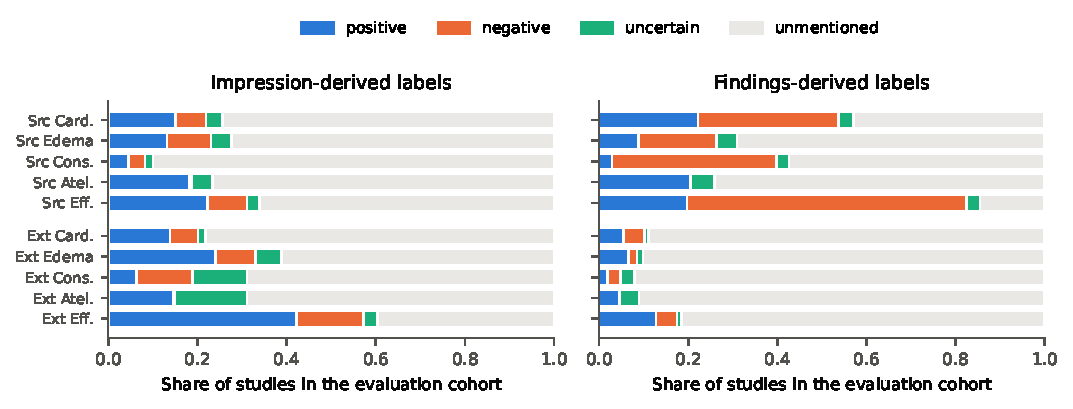
\includegraphics[width=\linewidth]{figures/fig2_label_composition.pdf}
\caption{Share of evaluation-cohort studies whose label for each target is
positive, negative, uncertain or unmentioned, by site and report section.
Values are in \cref{tab:labels}.}
\label{fig:labels}
\end{figure}

\subsection{The estimator defect and its correction}
\label{sec:res-defect}
Every original Stage 10 estimate was reproduced exactly from the cached
predictions. The original estimator counts each accepted study without a
labelled target as error-free, so its value is the error among evaluable
accepted studies multiplied by the evaluable fraction of accepted studies
(\cref{sec:endpoint}). That fraction is about 0.5 at the source and 0.8
externally, so the original estimator deflated source risk roughly twice as
much as external risk (\cref{tab:levels}). For M4 under intact context, the
original risks were \RiskOrigSrcMFour{} (source) and \RiskOrigExtMFour{}
(external); among evaluable studies they were \RiskEvalSrcMFour{} and
\RiskEvalExtMFour{}.

\begin{table}[t]
\centering\small
\caption{Selective error at the frozen 80\% cutoff under the original estimator
(label-less studies counted correct) and the corrected evaluable-study
estimator, with realised coverage over all eligible studies.}
\label{tab:levels}
\begin{adjustbox}{max width=\linewidth}
\begin{tabular}{llrrrrrr}
\toprule
 & & \multicolumn{3}{c}{Source} & \multicolumn{3}{c}{External}\\
\cmidrule(lr){3-5}\cmidrule(lr){6-8}
Model & Estimator & C0 & C1 & C2 & C0 & C1 & C2\\
\midrule
M1 & original (defective) & 0.1084 & 0.1084 & 0.1084 & 0.1818 & 0.1818 & 0.1818\\
 & evaluable-study & 0.2111 & 0.2111 & 0.2111 & 0.2230 & 0.2230 & 0.2230\\
 & \emph{coverage (all)} & 0.796 & 0.796 & 0.796 & 0.772 & 0.772 & 0.772\\
\addlinespace
M2 & original (defective) & 0.1575 & 0.2411 & 0.2415 & 0.2338 & 0.2605 & 0.2667\\
 & evaluable-study & 0.3042 & 0.4565 & 0.4618 & 0.2869 & 0.3203 & 0.3279\\
 & \emph{coverage (all)} & 0.803 & 1.000 & 0.790 & 0.847 & 1.000 & 0.846\\
\addlinespace
M3 & original (defective) & 0.1102 & 0.0951 & 0.1426 & 0.1571 & 0.1444 & 0.1676\\
 & evaluable-study & 0.1937 & 0.1755 & 0.2538 & 0.1895 & 0.1761 & 0.2024\\
 & \emph{coverage (all)} & 0.798 & 0.821 & 0.728 & 0.774 & 0.828 & 0.746\\
\addlinespace
M4 & original (defective) & 0.0744 & 0.0720 & 0.0893 & 0.1128 & 0.1200 & 0.1140\\
 & evaluable-study & 0.1391 & 0.1395 & 0.1695 & 0.1374 & 0.1466 & 0.1388\\
 & \emph{coverage (all)} & 0.800 & 0.805 & 0.789 & 0.795 & 0.764 & 0.788\\
\bottomrule
\end{tabular}

\end{adjustbox}
\end{table}

\subsection{Registered hypotheses}
\label{sec:res-hyp}
\Cref{tab:hyp} gives every Stage 10 contrast under both estimators with the
registered verdict rule. Under the corrected estimator, H1 was not confirmed
for either multimodal model: \HOneMThreeEval{} for M3 and \HOneMFourEval{} for
M4. Both intervals lie inside $(-0.02,0.02)$, so they exclude a material
increase at the realised calibration sample and model weights. Under the
original estimator the same contrasts were \HOneMThreeOrig{} and
\HOneMFourOrig{}, the original confirmation. H2 (C1) was not confirmed by
either estimator: \HTwoMThreeCOneEval{} for M3 and \HTwoMFourCOneEval{} for M4.
The registered H3 is identical to H2-C1 and is likewise not confirmed. The post
hoc transfer-gap version of H3 was negative for both models under both
estimators. Under the corrected estimator its magnitude is below materiality
(\HThreeMThreeEval{} and \HThreeMFourEval{}), so the ``reversal at
materiality'' of the previous draft does not survive correction.

Under its registered direction-only rule, H4 was supported for M3 at both sites
and for M4 at the source. For M4 externally, misaligned context gave lower
error than absent context (\HFourMFourexternalEval{}).

\begin{table}[t]
\centering\footnotesize
\begin{adjustbox}{max width=\linewidth}
\begin{tabular}{lllrlrl}
\toprule
H & Model & Contrast & \multicolumn{2}{c}{Original estimator} & \multicolumn{2}{c}{Corrected (evaluable-study)}\\
\cmidrule(lr){4-5}\cmidrule(lr){6-7}
 & & & Estimate (95\% CI) & V & Estimate (95\% CI) & V\\
\midrule
H1 & M3 & ext $-$ src, C0 & +0.0469 (+0.0408, +0.0531) & C & $-$0.0042 ($-$0.0145, +0.0061) & I\\
H1 & M4 & ext $-$ src, C0 & +0.0384 (+0.0336, +0.0430) & C & $-$0.0018 ($-$0.0108, +0.0064) & I\\
H2 & M3 & interaction, C1 & +0.0024 ($-$0.0027, +0.0076) & I & +0.0048 ($-$0.0038, +0.0134) & I\\
H2 & M4 & interaction, C1 & +0.0096 (+0.0048, +0.0144) & S & +0.0089 (+0.0002, +0.0173) & S\\
\midrule\multicolumn{7}{l}{\emph{H3 as coded after inspection (registered H3 $\equiv$ H2-C1)}}\\
H3 & M3 & gap $-$ gap(M1) & $-$0.0265 ($-$0.0321, $-$0.0212) & O [O*] & $-$0.0162 ($-$0.0256, $-$0.0070) & O [O]\\
H3 & M4 & gap $-$ gap(M1) & $-$0.0350 ($-$0.0408, $-$0.0292) & O [O*] & $-$0.0138 ($-$0.0243, $-$0.0029) & O [O]\\
\midrule\multicolumn{7}{l}{\emph{Secondary: H4 (direction only, no materiality)}}\\
H4 & M3 & C2 $-$ C1, source & +0.0475 (+0.0422, +0.0524) & C & +0.0783 (+0.0691, +0.0865) & C\\
H4 & M4 & C2 $-$ C1, source & +0.0173 (+0.0125, +0.0217) & C & +0.0301 (+0.0215, +0.0383) & C\\
H4 & M3 & C2 $-$ C1, external & +0.0231 (+0.0211, +0.0250) & C & +0.0263 (+0.0240, +0.0286) & C\\
H4 & M4 & C2 $-$ C1, external & $-$0.0060 ($-$0.0080, $-$0.0041) & O & $-$0.0077 ($-$0.0101, $-$0.0054) & O\\
\midrule\multicolumn{7}{l}{\emph{Not registered (computed by the original analysis code; descriptive)}}\\
H2 & M3 & interaction, C2 & $-$0.0219 ($-$0.0279, $-$0.0160) & O* & $-$0.0472 ($-$0.0572, $-$0.0374) & O*\\
H2 & M4 & interaction, C2 & $-$0.0137 ($-$0.0185, $-$0.0087) & O & $-$0.0289 ($-$0.0377, $-$0.0199) & O*\\
H1 & M1 & ext $-$ src, C0 & +0.0734 (+0.0668, +0.0802) & C & +0.0120 ($-$0.0002, +0.0244) & I\\
H1 & M2 & ext $-$ src, C0 & +0.0763 (+0.0687, +0.0838) & C & $-$0.0173 ($-$0.0292, $-$0.0054) & O\\
\bottomrule
\end{tabular}

\end{adjustbox}
\caption{All Stage 10 contrasts under the original and corrected estimators.
V: verdict under the registered rule (H1, H2: interval above zero and point
$\ge0.02$; H3: no materiality registered; H4: interval above zero). C
confirmed; S same direction, below materiality; I inconclusive (interval
includes zero); O opposite direction (below materiality, or no materiality
registered); O* opposite direction with magnitude $\ge0.02$. For H3 the bracket gives the verdict with the 0.02
materiality that the Stage 10 code applied. Rows marked not registered were
computed by the Stage 10 code but are not registered hypotheses.}
\label{tab:hyp}
\end{table}

\subsection{The cross-site contrast is not robust to defensible endpoint choices}
\label{sec:res-sensitivity}
\Cref{fig:spec} and \cref{tab:sens} show H1 under 15 specifications. Among
estimators that exclude label-less studies, the M4 transfer gap ranged from
\SensUncPosHOneMFour{} with uncertain labels counted as positive to
\SensUnmNegHOneMFour{} with unmentioned labels counted as negative. It was
\SensMacroHOneMFour{} under pathology-macro aggregation and
\SensFindHOneMFour{} with findings labels. Under the second training seed it was
\SensSeedHOneMFour{}, against \HOneMFourEval{} for the primary seed. The
original estimator gave \SensSeedOrigHOneMFour{} for that seed, which is why the
earlier replicate appeared to agree. For M3, retraining M2 under the second
seed (M3 averages M1 and M2) moved the corrected gap from \HOneMThreeEval{} to
\SensSeedHOneMThree{}. For M3, estimates ranged from
\SensTTenHOneMThreePt{} ($T=10$) to \SensUnmNegHOneMThreePt{} (unmentioned
counted as negative). No single factor dominated. Depending on the model, each
of the following moved the estimate by more than its own interval width:
aggregation (M1: \SensEvalHOneMOnePt{} evaluable-study against
\SensMacroHOneMOnePt{} pathology-macro), label handling (all models), label
source (M1 and M3) and training seed (M3 and M4).

The label-handling and aggregation specifications share the same predictions,
thresholds and cutoffs. Only which cells count as labelled, and how cells are
pooled, changes between them, and these choices alone decide the sign of the
cross-site contrast. Treating unmentioned cells
as negative brings the external site's lower specificity into view
(\cref{sec:res-operating}). The primary handling hides it, because labelled
external cells are mostly positive. Counting uncertain cells as positive does
the reverse for the same reason.

The pathology-specific contrasts that the original SAP made primary
(supplement) were heterogeneous. For M4 the primary labels gave cardiomegaly
\PathMFourCard{} and atelectasis \PathMFourAtel{}, while counting unmentioned as
negative made every pathology positive (\PathMFourUnmMin{} to
\PathMFourUnmMax{}). Restricted to AP-only studies, M4's
transfer gap was \ViewAPMFour{}; restricted to PA-only studies, \ViewPAMFour{}.
AP-only studies made up \APShareSrc{} of the source cohort and \APShareExt{} of
the external one, so view mix also enters the aggregate contrast.

\begin{figure}[t]
\centering
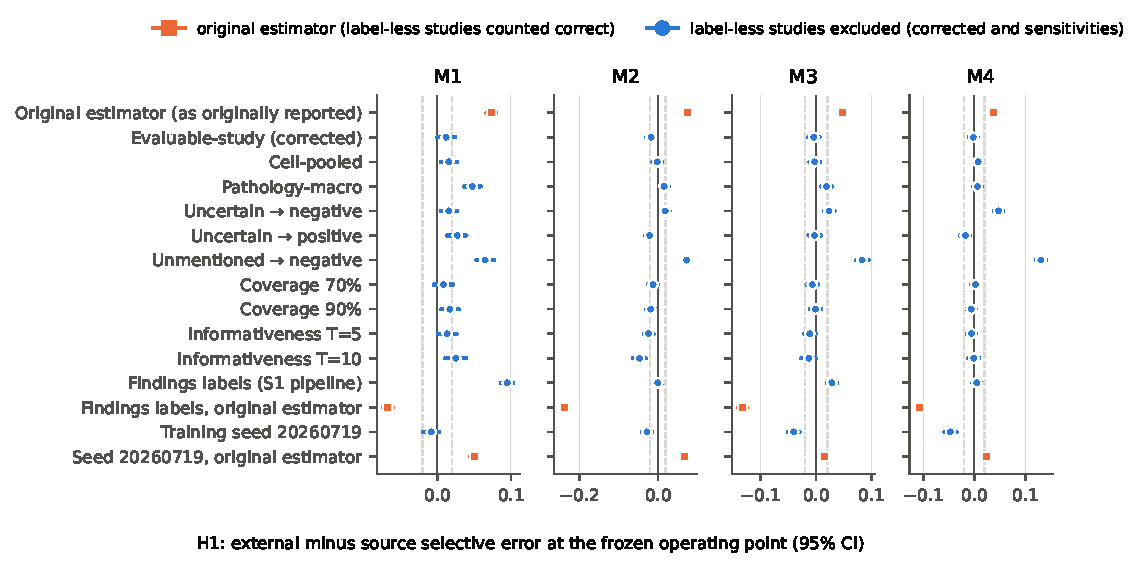
\includegraphics[width=\linewidth]{figures/fig1_h1_specifications.pdf}
\caption{H1 transfer gap (external minus source selective error, 95\% CI) for
each model under 15 specifications. Label-handling and aggregation rows share
the primary predictions, thresholds and cutoffs. Coverage rows change the
cutoff, $T$ rows the cohort, findings rows the labels, cohort and thresholds, and
seed rows the models. Square markers use the original estimator, which counts studies
without a labelled target as correct. Dashed lines mark $\pm0.02$. Values are
in \cref{tab:sens} and the supplement.}
\label{fig:spec}
\end{figure}

\begin{table}[t]
\centering\scriptsize
\caption{H1 and the post hoc transfer-gap H3 for the multimodal models across
specifications (point estimate and 95\% CI). Label-handling and aggregation rows
hold the primary predictions, thresholds and cutoffs fixed; the other rows change
the cutoff (coverage), the cohort ($T$), the labels, cohort and thresholds
(findings) or the models (seed).}
\label{tab:sens}
\begin{adjustbox}{max width=\linewidth}
\begin{tabular}{lrrrr}
\toprule
Specification & H1 M3 & H1 M4 & H3 M3 & H3 M4\\
\midrule
Original estimator (as originally reported) & +0.0469 (+0.041, +0.053) & +0.0384 (+0.034, +0.043) & $-$0.0265 ($-$0.032, $-$0.021) & $-$0.0350 ($-$0.041, $-$0.029)\\
Evaluable-study (corrected) & $-$0.0042 ($-$0.014, +0.006) & $-$0.0018 ($-$0.011, +0.006) & $-$0.0162 ($-$0.026, $-$0.007) & $-$0.0138 ($-$0.024, $-$0.003)\\
Cell-pooled & $-$0.0026 ($-$0.012, +0.007) & +0.0076 ($-$0.000, +0.015) & $-$0.0183 ($-$0.026, $-$0.010) & $-$0.0080 ($-$0.017, +0.001)\\
Pathology-macro & +0.0188 (+0.009, +0.029) & +0.0063 ($-$0.002, +0.014) & $-$0.0287 ($-$0.037, $-$0.020) & $-$0.0412 ($-$0.050, $-$0.032)\\
Uncertain $\to$ negative & +0.0232 (+0.014, +0.033) & +0.0475 (+0.039, +0.056) & +0.0075 ($-$0.001, +0.016) & +0.0319 (+0.022, +0.042)\\
Uncertain $\to$ positive & $-$0.0025 ($-$0.014, +0.008) & $-$0.0176 ($-$0.027, $-$0.009) & $-$0.0295 ($-$0.038, $-$0.020) & $-$0.0446 ($-$0.055, $-$0.034)\\
Unmentioned $\to$ negative & +0.0828 (+0.072, +0.094) & +0.1306 (+0.121, +0.141) & +0.0179 (+0.013, +0.023) & +0.0657 (+0.059, +0.073)\\
Coverage 70\% & $-$0.0069 ($-$0.017, +0.003) & +0.0029 ($-$0.006, +0.011) & $-$0.0150 ($-$0.025, $-$0.005) & $-$0.0052 ($-$0.016, +0.006)\\
Coverage 90\% & $-$0.0010 ($-$0.011, +0.009) & $-$0.0058 ($-$0.015, +0.002) & $-$0.0181 ($-$0.027, $-$0.009) & $-$0.0229 ($-$0.033, $-$0.012)\\
Informativeness $T=5$ & $-$0.0114 ($-$0.022, $-$0.001) & $-$0.0057 ($-$0.015, +0.003) & $-$0.0248 ($-$0.034, $-$0.015) & $-$0.0190 ($-$0.030, $-$0.008)\\
Informativeness $T=10$ & $-$0.0130 ($-$0.027, $-$0.000) & $-$0.0009 ($-$0.012, +0.010) & $-$0.0381 ($-$0.050, $-$0.026) & $-$0.0260 ($-$0.039, $-$0.012)\\
Findings labels (S1 pipeline) & +0.0285 (+0.019, +0.038) & +0.0048 ($-$0.003, +0.013) & $-$0.0666 ($-$0.074, $-$0.058) & $-$0.0903 ($-$0.098, $-$0.082)\\
Findings labels, original estimator & $-$0.1324 ($-$0.140, $-$0.125) & $-$0.1079 ($-$0.114, $-$0.101) & $-$0.0652 ($-$0.071, $-$0.058) & $-$0.0408 ($-$0.047, $-$0.034)\\
Training seed 20260719 & $-$0.0402 ($-$0.050, $-$0.030) & $-$0.0469 ($-$0.059, $-$0.035) & $-$0.0320 ($-$0.040, $-$0.024) & $-$0.0386 ($-$0.047, $-$0.030)\\
Seed 20260719, original estimator & +0.0145 (+0.009, +0.021) & +0.0246 (+0.018, +0.031) & $-$0.0366 ($-$0.041, $-$0.032) & $-$0.0265 ($-$0.032, $-$0.022)\\
\bottomrule
\end{tabular}

\end{adjustbox}
\end{table}

\subsection{Controlled label-source decomposition}
\label{sec:res-label-source}
The original findings-label sensitivity (S1) changed the label set, the
source cohort (14,766 to 9,293 studies), the thresholds and cutoffs (re-selected
on findings calibration labels), and the C2 donor realisation, all at once.
Model parameters did not change. External probabilities agreed between the two
runs to within \SOneMaxProbDiff{}. With S1's re-selected thresholds, however,
M1's external decisions differed in \SOneMOneCells{} cells and its acceptance in
\SOneMOneStudies{} studies, and across models \SOneCellsChanged{} cells and
\SOneStudiesChanged{} studies changed. The previous draft's argument that ``only
the labels differ'' for the image-only control was therefore incorrect.
\Cref{tab:ls} changes one factor at a time.

Swapping labels alone (A0$\to$A1) on the same studies, with identical
decisions and accepted sets, moved the original-estimator M3 contrast from
\LSAZeroMThreeOrig{} to \LSAOneMThreeOrig{}. Restricting the source cohort
(A1$\to$A2) moved it further, to \LSATwoMThreeOrig{}, because it removes
label-less source studies that the original estimator counted as correct.
Re-selecting thresholds (A2$\to$A3) reproduced the originally reported
\LSAThreeMThreeOrig{}. Under the corrected estimator the cohort restriction has
exactly no effect, because the removed studies are not evaluable under findings
labels. The remaining movement is shared between labels (A0$\to$A1:
\LSAZeroMThreeEval{} to \LSAOneMThreeEval{} for M3, and \LSAZeroMFourEval{} to
\LSAOneMFourEval{} for M4) and thresholds (A2$\to$A3: to \LSAThreeMThreeEval{} and
\LSAThreeMFourEval{}). On cells labelled under both sources (A1c), impression and
findings labels gave nearly the same contrasts: \LSAOnecIMThreeEval{} and
\LSAOnecFMThreeEval{} for M3. Under the corrected estimator, the findings-label
result does not reverse the primary; for M3 it points in the hypothesised
direction. The originally reported reversal under S1 was produced by the estimator defect
interacting with the asymmetric cohort definition, not by the label sets
measuring opposite things.

\begin{table}[t]
\centering\scriptsize
\caption{Controlled label-source decomposition of H1 (point estimates; intervals
in the supplement). Evaluable studies: share of each cohort with at least one
labelled target under that step's labels. Under the corrected estimator, A2
equals A1 because the studies removed by the cohort restriction are not
evaluable under findings labels.}
\label{tab:ls}
\begin{adjustbox}{max width=\linewidth}
\begin{tabular}{llrrrrrr}
\toprule
 & & \multicolumn{2}{c}{Evaluable studies} & \multicolumn{2}{c}{H1 M3} & \multicolumn{2}{c}{H1 M4}\\
\cmidrule(lr){3-4}\cmidrule(lr){5-6}\cmidrule(lr){7-8}
Step & Change from A0 & Src & Ext & Original & Corrected & Original & Corrected\\
\midrule
A0 & primary (impression labels, primary cohort, impression thresholds) & 53\% & 81\% & +0.0469 & $-$0.0042 & +0.0384 & $-$0.0018\\
A1 & findings labels only & 59\% & 24\% & $-$0.0613 & +0.0090 & $-$0.0839 & $-$0.0389\\
A1c-I & common labelled cells, impression labels & 20\% & 17\% & $-$0.0059 & $-$0.0042 & $-$0.0065 & $-$0.0212\\
A1c-F & common labelled cells, findings labels & 20\% & 17\% & $-$0.0069 & $-$0.0090 & $-$0.0077 & $-$0.0271\\
A2x & findings cohort only & 37\% & 81\% & +0.0809 & +0.0012 & +0.0664 & +0.0126\\
A2 & findings cohort + labels & 94\% & 24\% & $-$0.1359 & +0.0090 & $-$0.1610 & $-$0.0389\\
A3 & + findings thresholds and cutoffs (= original S1) & 94\% & 24\% & $-$0.1324 & +0.0285 & $-$0.1079 & +0.0048\\
B2 & findings labels + thresholds, primary cohort & 59\% & 24\% & $-$0.0579 & +0.0285 & $-$0.0524 & +0.0048\\
\bottomrule
\end{tabular}

\end{adjustbox}
\end{table}

\subsection{Frozen thresholds and per-pathology operating points}
\label{sec:res-operating}
Aggregate error hid a shift in operating points (\cref{tab:operating},
\cref{fig:operating}). For M4 among accepted studies, cardiomegaly specificity
fell from \MFourCardSpecSrc{} at the source to \MFourCardSpecExt{} externally
while sensitivity rose from \MFourCardSensSrc{} to \MFourCardSensExt{}. The
model called cardiomegaly in \MFourCardPosSrc{} of accepted studies at the
source and \MFourCardPosExt{} externally. Specificity also fell for effusion
(\MFourEffSpecSrc{} to \MFourEffSpecExt{}) and edema (\MFourEdemaSpecSrc{} to
\MFourEdemaSpecExt{}). Negative labels are explicit mentions and therefore a
selected subset, so these specificities carry verification bias. The direction
held when unmentioned cells were counted as negative (supplement). A frozen
threshold transferred a decision rule, not an operating point.

\begin{table}[t]
\centering\scriptsize
\caption{Per-pathology operating characteristics among accepted studies (C0),
labelled cells only. Pos.\ call: share of accepted studies in which the model
called the finding positive.}
\label{tab:operating}
\begin{adjustbox}{max width=\linewidth}
\begin{tabular}{lllrrrrrr}
\toprule
 & & & \multicolumn{3}{c}{Source} & \multicolumn{3}{c}{External}\\
\cmidrule(lr){4-6}\cmidrule(lr){7-9}
Model & Pathology & $t_j$ & Sens. & Spec. & Pos.\ call & Sens. & Spec. & Pos.\ call\\
\midrule
M3 & Cardiomegaly & 0.617 & 0.872 & 0.788 & 0.585 & 0.965 & 0.579 & 0.704\\
 & Edema & 0.575 & 0.840 & 0.806 & 0.389 & 0.808 & 0.749 & 0.539\\
 & Consolidation & 0.553 & 0.824 & 0.851 & 0.416 & 0.808 & 0.905 & 0.591\\
 & Atelectasis & 0.986 & 0.667 & 0.780 & 0.451 & 0.550 & 0.897 & 0.515\\
 & Pleural Effusion & 0.686 & 0.863 & 0.841 & 0.448 & 0.851 & 0.901 & 0.589\\
\addlinespace
M4 & Cardiomegaly & 0.633 & 0.887 & 0.823 & 0.563 & 0.972 & 0.438 & 0.756\\
 & Edema & 0.436 & 0.848 & 0.838 & 0.363 & 0.885 & 0.653 & 0.651\\
 & Consolidation & 0.584 & 0.841 & 0.889 & 0.376 & 0.805 & 0.915 & 0.531\\
 & Atelectasis & 0.964 & 0.886 & 0.460 & 0.724 & 0.911 & 0.498 & 0.875\\
 & Pleural Effusion & 0.798 & 0.870 & 0.887 & 0.487 & 0.950 & 0.641 & 0.751\\
\bottomrule
\end{tabular}

\end{adjustbox}
\end{table}

\begin{figure}[t]
\centering
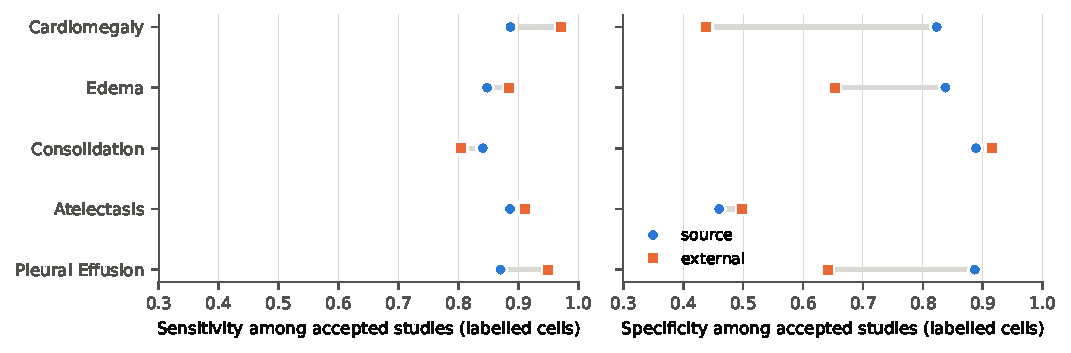
\includegraphics[width=\linewidth]{figures/fig4_operating_points.pdf}
\caption{M4 sensitivity and specificity among accepted studies at the source
(circles) and external site (squares), labelled cells only. Values in
\cref{tab:operating}.}
\label{fig:operating}
\end{figure}

\subsection{Coverage, the confidence score and alternative policies}
\label{sec:res-selective}
With context intact, realised coverage stayed within \CovDriftMaxCZero{} of the
80\% target for every model at both sites, and within \SeedCovDriftMax{} under
the second seed. Under intervention it moved: M2 under C1 accepted every study
at both sites (\MTwoCOneCovSrc{} and \MTwoCOneCovExt{}), because a constant
placeholder makes its output constant and every study ties at the same
confidence. M3 under C2 fell to \MThreeCTwoCovSrc{} and \MThreeCTwoCovExt{}.
Coverage held while per-pathology operating points shifted
(\cref{sec:res-operating}), so coverage monitoring alone would not reveal that
shift. Whether selective \emph{error} degraded is the question the labels could
not settle (\cref{sec:res-sensitivity}).

The frozen confidence score ranked study-level correctness only weakly:
failure-detection AUROC was \FailAUROCFrozenMin{}--\FailAUROCFrozenMax{} across
models and sites (\cref{fig:rc}, \cref{tab:comparators}). Three comparators
were fitted on the source calibration tier only. A per-pathology
temperature-scaled margin left the policy nearly unchanged. A decision-aware
expected-loss score, built from Platt-calibrated probabilities of error for the
decisions actually made, ranked errors better (AUROC
\FailAUROCELMin{}--\FailAUROCELMax{}) and lowered risk at both sites. Its
operating point transported worse: M4's external coverage was \ELMFourExtCov{}
against an 80\% calibration target. Split-conformal singleton acceptance with
one miscoverage level could not reach 80\% calibration coverage
(\ConfAccMin{}--\ConfAccMax{}), because near-uniformly positive atelectasis
labels make that pathology's sets rarely singleton. Its acceptance rate also
moved at the external site.

\begin{figure}[t]
\centering
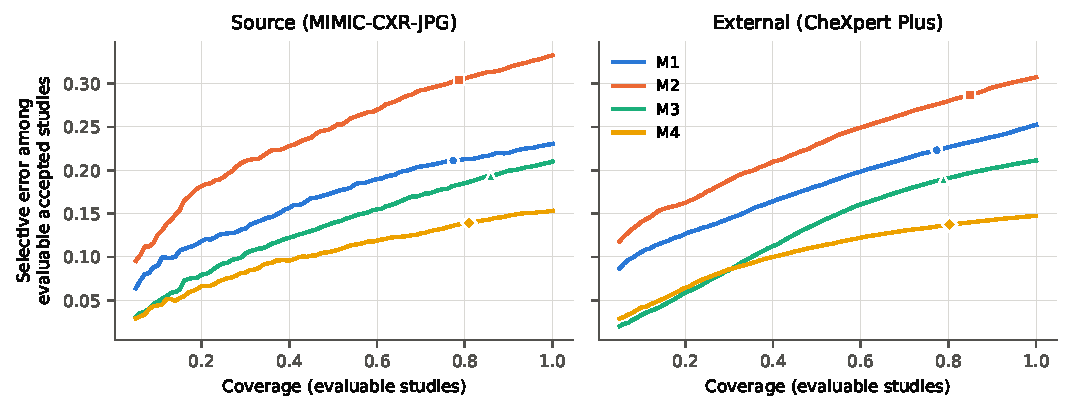
\includegraphics[width=\linewidth]{figures/fig3_risk_coverage.pdf}
\caption{Risk--coverage curves over evaluable studies (C0), ranking by the
frozen confidence score. Markers show the frozen 80\% operating point at its
realised coverage among evaluable studies.}
\label{fig:rc}
\end{figure}

\begin{table}[t]
\centering\scriptsize
\caption{Alternative selective policies (post hoc), all fitted on the source
calibration tier and applied unchanged. Failure AUROC: discrimination of
studies with no error versus any error, evaluable studies. H1 corrected:
evaluable-study transfer gap.}
\label{tab:comparators}
\begin{adjustbox}{max width=\linewidth}
\begin{tabular}{llrrrrrr}
\toprule
 & & \multicolumn{2}{c}{Coverage (C0)} & \multicolumn{2}{c}{Failure AUROC} & & \\
\cmidrule(lr){3-4}\cmidrule(lr){5-6}
Model & Policy & Src & Ext & Src & Ext & H1 corrected (95\% CI) & Ext.\ coverage C1\\
\midrule
M3 & Frozen (|2p$-$1|) & 0.798 & 0.774 & 0.632 & 0.648 & $-$0.0042 ($-$0.014, +0.006) & 0.828\\
 & Temperature-scaled margin & 0.798 & 0.772 & 0.633 & 0.652 & $-$0.0042 ($-$0.015, +0.006) & 0.827\\
 & Expected-loss (decision-aware) & 0.797 & 0.733 & 0.738 & 0.746 & $-$0.0166 ($-$0.026, $-$0.007) & 0.777\\
 & Split-conformal singletons & 0.515 & 0.552 & 0.643 & 0.697 & $-$0.0205 ($-$0.029, $-$0.013) & 0.572\\
\addlinespace
M4 & Frozen (|2p$-$1|) & 0.800 & 0.795 & 0.625 & 0.603 & $-$0.0018 ($-$0.011, +0.006) & 0.764\\
 & Temperature-scaled margin & 0.800 & 0.796 & 0.627 & 0.604 & $-$0.0018 ($-$0.011, +0.006) & 0.762\\
 & Expected-loss (decision-aware) & 0.800 & 0.855 & 0.704 & 0.687 & +0.0056 ($-$0.002, +0.013) & 0.937\\
 & Split-conformal singletons & 0.559 & 0.693 & 0.644 & 0.664 & +0.0290 (+0.021, +0.037) & 0.701\\
\bottomrule
\end{tabular}

\end{adjustbox}
\end{table}

\subsection{Context interventions within each site}
\label{sec:res-context}
For M3, misaligned context (C2) gave higher error than absent context (C1) at
the source under every estimator, label variant, coverage, informativeness
threshold, label source, C2 permutation and both training seeds
(\HFourMThreesourceEval{} for the primary seed, \RepTwoHFourMThreesourceeval{}
for the second). At the external site it did so under every specification for
the primary seed (\HFourMThreeexternalEval{}), and an alternative C2 donor
permutation left it essentially unchanged (range \PermHFourMThreeExtRange{}
across the two permutations). Under the second training seed the
corrected estimate was \RepTwoHFourMThreeexternaleval{}, inconclusive, and the
original estimator gave \RepTwoHFourMThreeexternalorig{}. For M4 the effect was positive at the
source (\HFourMFoursourceEval{}) in all primary-seed specifications, but the
interval included zero under the second seed. Externally its sign depended on
label handling. Removing or replacing context mostly changed predictions rather
than selection (\cref{tab:context}). Even so, the accepted sets under C0 and
under intervention overlapped only partially (Jaccard
\JaccardMin{}--\JaccardMax{}), so paired conditions do not evaluate the same
accepted studies. The two orderings of the selection/prediction split
disagreed by up to \OrderGapMM{} for the multimodal models (\OrderGapMTwo{} for M2), so no unique
additive split exists. The C2
interaction was negative for both multimodal models under the primary labels
(\HTwoMThreeCTwoEval{} and \HTwoMFourCTwoEval{}), meaning misalignment cost less
externally. This is consistent with the shorter external contexts (mean
\CTwoTokensExt{} versus \CTwoTokensSrc{} effective tokens), of which C2 changed
the target-term content in \CTwoTermDiffExt{} of external rows against
\CTwoTermDiffSrc{} at the source. The C2 interaction is not a registered
hypothesis, and its sign reversed when unmentioned cells were counted as
negative.

\begin{table}[t]
\centering\scriptsize
\caption{Selection versus prediction under context interventions (corrected
estimator). Policy effect $=R_c(A_c)-R_0(A_0)$; prediction on C0 set
$=R_c(A_0)-R_0(A_0)$; selection (o1) $=R_c(A_c)-R_c(A_0)$; selection (o2)
$=R_0(A_c)-R_0(A_0)$; Jaccard overlap of $A_0$ and $A_c$. Intervals in the
supplement.}
\label{tab:context}
\begin{adjustbox}{max width=\linewidth}
\begin{tabular}{lllrrrrr}
\toprule
Site & Model & Cond. & Policy effect & Pred.\ on C0 set & Selection (o1) & Selection (o2) & Jaccard\\
\midrule
source & M3 & C1 & $-$0.0182 & $-$0.0181 & $-$0.0001 & +0.0075 & 0.69\\
 & M3 & C2 & +0.0601 & +0.0714 & $-$0.0113 & +0.0148 & 0.64\\
 & M4 & C1 & +0.0003 & +0.0000 & +0.0003 & +0.0054 & 0.68\\
 & M4 & C2 & +0.0304 & +0.0333 & $-$0.0029 & +0.0079 & 0.68\\
\addlinespace
external & M3 & C1 & $-$0.0134 & $-$0.0127 & $-$0.0007 & +0.0063 & 0.68\\
 & M3 & C2 & +0.0129 & +0.0157 & $-$0.0029 & +0.0077 & 0.67\\
 & M4 & C1 & +0.0092 & +0.0132 & $-$0.0040 & +0.0011 & 0.65\\
 & M4 & C2 & +0.0015 & +0.0031 & $-$0.0017 & +0.0002 & 0.68\\
\bottomrule
\end{tabular}

\end{adjustbox}
\end{table}

\subsection{Sources of uncertainty the evaluation bootstrap omits}
\label{sec:res-uncertainty}
Resampling calibration patients and re-applying the frozen selection rule moved
the corrected H1 estimates with a standard deviation \CalRatioMin{}--\CalRatioMax{}
times the evaluation-bootstrap standard deviation (\cref{tab:uncertainty}). For
M4 the calibration standard deviation was \CalSDMFour{} against \EvalSDMFour{}, and
per-pathology thresholds varied with standard deviation up to \ThrSDMaxMFour{}.
The training seed moved the corrected H1 of both multimodal models by about
0.04 (\cref{sec:res-sensitivity}). The reported intervals, which condition on
one calibration sample and one training run, therefore understate total
uncertainty substantially for cross-site contrasts.

\begin{table}[t]
\centering\scriptsize
\caption{H1 variability from resampling evaluation patients (bootstrap SD,
approximated from the 95\% interval) and from resampling calibration patients
with the frozen selection rule re-applied (200 replicates).}
\label{tab:uncertainty}
\begin{adjustbox}{max width=\linewidth}
\begin{tabular}{llrrrr}
\toprule
Model & Estimator & H1 & SD (evaluation bootstrap) & SD (calibration resample) & Calibration 2.5--97.5\%\\
\midrule
M1 & original & +0.0734 & 0.0034 & 0.0044 & (+0.0635, +0.0845)\\
 & evaluable-study & +0.0120 & 0.0063 & 0.0092 & ($-$0.0003, +0.0388)\\
M2 & original & +0.0763 & 0.0038 & 0.0067 & (+0.0740, +0.0984)\\
 & evaluable-study & $-$0.0173 & 0.0061 & 0.0205 & ($-$0.0254, +0.0408)\\
M3 & original & +0.0469 & 0.0031 & 0.0050 & (+0.0352, +0.0554)\\
 & evaluable-study & $-$0.0042 & 0.0053 & 0.0097 & ($-$0.0271, +0.0141)\\
M4 & original & +0.0384 & 0.0024 & 0.0032 & (+0.0316, +0.0440)\\
 & evaluable-study & $-$0.0018 & 0.0044 & 0.0102 & ($-$0.0286, +0.0102)\\
\bottomrule
\end{tabular}

\end{adjustbox}
\end{table}

\subsection{Integrity checks and exploratory strata}
\label{sec:res-c2}
The previous draft reported 6 source and 34 external studies ``retaining their
own context'' under C2. Replaying the assignment, verified to reproduce it
exactly, showed that every one of these rows received identical text donated by
a \emph{different} patient. No recipient received context from its own patient
(\CTwoSamePatSrc{} and \CTwoSamePatExt{} same-patient donors). The count was a
count of identical boilerplate, not of constraint violations. Image-only
predictions were identical across conditions at both sites.

Among external demographic groups (exploratory; no source demographics were
available), M4's coverage differed by at most \AgeCovDispMFour{} across age bands
and \InsCovDispMFour{} across insurance categories. M3's coverage differed by \AgeCovDispMThree{}
across age bands, which exceeds the 0.05 drift materiality (supplement). These
are single-site, post hoc descriptions with no cross-site comparison.

\section{Discussion}
\label{sec:discussion}

\subsection{Principal findings}
The preregistered transport-failure hypothesis was not confirmed once a
verified estimator defect was corrected. The original analysis counted every
accepted study whose report mentioned none of the five targets as correctly
classified. Such studies were about half of the source cohort and a fifth of
the external one, so the originally reported transfer gaps of about 0.04--0.05 for the
multimodal models measured the difference in label availability between the two
report corpora rather than a change in model error. Over studies with at least
one labelled target, the multimodal transfer gaps were close to zero. Their
intervals excluded a material increase, conditional on the realised calibration
sample and training run (\cref{sec:res-uncertainty}).

That near-zero estimate is itself fragile. With predictions and frozen
thresholds held fixed, plausible choices about uncertain and unmentioned
labels, the report section used for labels, aggregation across pathologies, the
training seed and the view stratum each moved the cross-site contrast by more
than its interval width, and several changed its sign. The originally reported
findings-label ``reversal'' was produced mainly by the same defect acting on an
asymmetric cohort definition. Where both report sections label the same cell
they agree in more than 95\% of cases. Under the primary label handling, the
cross-site contrast is therefore not identified well enough to support a claim
in either direction.

Three results were more stable. Frozen per-pathology thresholds transferred a
decision rule but not an operating point: at the external site the feature-fusion
model called cardiomegaly, effusion and edema far more often, and its
specificity fell, under both label handlings examined. Realised coverage stayed
close to target with context intact, under both training seeds. Misaligned
context was worse than absent context for the late-fusion model at the source
under every specification and both seeds. Externally it held for the first seed
only.

\subsection{What the endpoint measured}
The selective-risk endpoint is an error rate over the cells a report labeller
chose to label, in the studies a policy accepted. Three distinct mechanisms can
change it between hospitals, and the data separate them only partly.
\emph{Case mix} differs: with unmentioned counted as negative, effusion and
edema are roughly twice as prevalent externally. \emph{Documentation practice}
differs. Source impressions omit all five targets in about half of studies, and
external impressions carry many more uncertain mentions. The findings section
records explicit negatives at the source but is absent from most external
studies. \emph{Labeller error} may differ too. The two sites were labelled by
CheXbert, but the external labels were produced by the dataset's publishers
with undocumented settings, and agreement between report labels and image
findings is imperfect~\cite{jain2021visualchexbert,rafferty2025limitations}.
Similar aggregate positive rates (\PosSrcImpression{} and \PosExtImpression{})
did not establish comparable labels, and different prevalence alone would not
have shown different disease definitions. What the controlled analysis does
establish is that selective missingness, meaning which cells and studies carry
a label at all, was the dominant driver of the originally reported cross-site contrast
and remains a first-order driver after correction.

\subsection{Implications for cross-site benchmarking}
The defect is easy to make and invisible in aggregate output. Any per-study
loss averaged over observed labels needs a convention for studies with none,
and a guard against division by zero silently chose one here. We suggest
the following checks for any cross-site evaluation built on report-derived
labels. Report, per site, the fraction of studies and of accepted studies
with at least one labelled target. Define and test the estimator's treatment
of unlabelled studies. Fix uncertain- and unmentioned-label handling in
advance and report the alternatives. Report pathology-specific operating
characteristics, not only aggregate error. Verify the unit at which a context
intervention is applied, and replay it to confirm its constraints. Quantify
calibration-sample uncertainty alongside the evaluation bootstrap. Where a
cross-site sign matters, obtain a reference standard that is dense and
comparable at both sites.

\subsection{Implications for deployment}
On this evidence a frozen threshold should not be assumed to keep its
operating point at a new hospital, even when its coverage holds. We did not
evaluate target-site recalibration: the protocol prohibits external tuning,
and recalibration answers a different question, whether a method can be
re-tuned rather than whether a shipped policy transports. We therefore make
no claim about whether recalibration would hide or restore any particular
failure. A decision-aware confidence score ranked errors better than the frozen
margin but held its coverage less well across sites. Better ranking at the
source did not make the operating point more transportable.

\subsection{Limitations}
\label{sec:limitations}
\emph{Labels.} All labels are automatic and report-derived. No expert
reference standard was available, and the endpoint is not a clinical
five-disease error rate. The external labels' generation settings are
undocumented. The decisive limitation for cross-site claims is that neither
label source is dense and comparable at both sites. We provide a blinded
adjudication protocol (supplement) as the route to resolving it; no
adjudication has been performed.

\emph{Post hoc analyses.} The estimator correction and every analysis labelled
R1 were done after the external results had been inspected. The correction
fixes a verified defect, but it reverses the original conclusion, and readers
should weigh it with that history in mind. Both estimators are reported. The
H3 operationalisation, the S1 implementation choices and the second training
seed were also decided after inspection.

\emph{Uncertainty.} Reported intervals condition on one calibration sample,
one C2 realisation and one training run per model. Two training seeds were
examined for every model. Calibration-sample
variability was \CalRatioMin{}--\CalRatioMax{} times the evaluation-bootstrap variability for the
corrected contrasts. Two seeds cannot establish that any result is
seed-independent. The second seed changed both multimodal models' corrected
transfer gaps by about 0.04, and removed M3's external context effect.

\emph{Interventions.} C2 was applied per image, and its donors depend on the
cohort being permuted. Removing context synthetically (C1) is not the same as
context that is naturally missing. The informativeness rule measures length,
not clinical content.

\emph{Scope.} One pair of hospitals in one direction. No compatible third
site with pre-diagnostic text and comparable labels was available to us.
Reverse transfer would require training on the external site, which the
protocol does not authorise. Demographic analyses are external-only and
exploratory because source demographics were not acquired. Images differ in
compression history at origin, although preprocessing was identical.

\emph{Protocol.} Two planning documents were written on 18 July 2026 before
any data access: a prose hypothesis registry and statistical analysis plan,
and the machine-readable registry that governed execution. The prose plan led
with AURC and pathology-specific reporting and required AP/PA, one-image,
concordant-study and uncertain-label sensitivities, and it was never formally
retired. The machine-readable registry required temperature-scaled and
split-conformal baselines and listed AUGRC as a primary threshold-free metric.
None of these was run before the results were known. Several are reported here
post hoc; the one-image-per-study and concordant-study sensitivities remain
unrun, because they need image-level predictions that were not cached.

\subsection{Future work}
The most informative next step is expert adjudication of a stratified sample
of studies at both sites, against which the label-handling alternatives can be
calibrated. A third institution with pre-diagnostic text would turn one
difference into a distribution. An informativeness rule based on clinical
content rather than length would make the context interaction interpretable.
Further training seeds for all four models would bound training variability.

\section{Conclusion}
A selective policy frozen at one hospital kept its coverage at another, but
its per-pathology operating points moved. Whether its selective error rose
could not be determined from report-derived labels whose availability differs
between the hospitals. The original conclusion that it rose was an artifact
of counting label-less studies as correct. A compound-shift protocol can
isolate context effects within a site, but cross-site risk claims require a
label endpoint that is comparable across sites. That requirement should be
established before such claims are made.


\section*{Protocol history and preregistration}
The record below is reconstructed from the project's version-control history,
the protocol amendment log and the stage artifacts. Commit times are recorded
by the authors' own system. Content hashes establish that a file existed in a
given form, not when it was written, and we know of no independently
time-stamped registration. The history is therefore offered as an auditable
account, not as independent proof of timing.

\begin{center}\small
\begin{tabular}{p{0.2\linewidth}p{0.74\linewidth}}
\toprule
Date (UTC+6) & Event\\
\midrule
18 Jul 2026, 17:14 & Prose hypothesis registry (H1--H6, AURC-led, pathology-specific) and statistical analysis plan committed; no data accessed.\\
18 Jul 2026, 22:38 & Machine-readable registry v0.1.0 (H1--H4, selective risk at the frozen cutoff, 0.02 materiality) committed; this registry governed execution. The prose documents were not formally retired.\\
28 Jul 2026 & v0.2.0 (context mapping, informativeness rule, structural exclusions) and v0.3.0 (prespecified evaluation partition; power clarification); no labels, models or external results existed.\\
3--4 Aug 2026 & v0.4.0--v0.4.2 (backbones, precision, learning rates); M1 had been trained and its internal-validation AUROC seen before v0.4.2.\\
6 Aug 2026 & Decision-rule and bootstrap code committed, including the H4 direction-only rule.\\
7 Aug 2026, 08:15 & External point estimates first inspected.\\
7 Aug 2026, 15:08 & Contrast code committed: H3 as transfer-gap difference; interaction under C2 (post hoc).\\
7 Aug 2026, 18:11 & S1 implemented with re-selected thresholds and a findings-restricted source cohort (post hoc implementation of a registered sensitivity).\\
8--21 Aug 2026 & $T=5,10$ sensitivities run; second training seed (M1, M4) decided, trained and analysed (not prespecified).\\
6--7 Oct 2026 & Revision R1: audit, estimator correction, and all analyses labelled R1, including M2 retrained under the second seed and the M2/M3 replicate (post hoc).\\
\bottomrule
\end{tabular}
\end{center}

The previous draft stated that the second training seed was prespecified and
that no amendment followed inspection of external results. The first statement
was incorrect. The registry names only a conditional three-seed ensemble. The
second statement was true of the amendment log but omitted the post-inspection
analysis decisions listed above, which are now recorded in that log
retrospectively.


\section*{Data and code availability}
MIMIC-CXR-JPG v2.1.0 and CheXpert Plus are available to credentialed
researchers from PhysioNet and Stanford AIMI respectively; neither is
redistributed. The protocol registry, all analysis code (including the
revision package \texttt{c3e.revision}), executable commands, tests, and every
aggregate artifact cited here are in the project repository
\authorinput{public repository URL and archived release DOI}. Row-level labels,
predictions, checkpoints and images remain in the protected data environment
required by the data use agreements.

\section*{Ethics}
\authorinput{state the ethics determination for secondary analysis of these
de-identified, credentialed-access datasets (e.g. institutional review or
exemption, and the PhysioNet and Stanford AIMI data use agreements under which
the authors accessed the data). No statement is supplied here because none has
been verified.}

\section*{Funding}
\authorinput{funding sources, or a statement that there was none}

\section*{Competing interests}
\authorinput{competing interests of each author}

\section*{Author contributions}
\authorinput{contributions of each author (e.g. CRediT roles); the repository
history does not establish individual contributions}

\section*{Acknowledgements}
\authorinput{optional}

\bibliographystyle{unsrt}
\bibliography{references_revised}

\end{document}
